\documentclass[twoside]{book}

% Packages required by doxygen
\usepackage{fixltx2e}
\usepackage{calc}
\usepackage{doxygen}
\usepackage[export]{adjustbox} % also loads graphicx
\usepackage{graphicx}
\usepackage[utf8]{inputenc}
\usepackage{makeidx}
\usepackage{multicol}
\usepackage{multirow}
\PassOptionsToPackage{warn}{textcomp}
\usepackage{textcomp}
\usepackage[nointegrals]{wasysym}
\usepackage[table]{xcolor}

% Font selection
\usepackage[T1]{fontenc}
\usepackage[scaled=.90]{helvet}
\usepackage{courier}
\usepackage{amssymb}
\usepackage{sectsty}
\renewcommand{\familydefault}{\sfdefault}
\allsectionsfont{%
  \fontseries{bc}\selectfont%
  \color{darkgray}%
}
\renewcommand{\DoxyLabelFont}{%
  \fontseries{bc}\selectfont%
  \color{darkgray}%
}
\newcommand{\+}{\discretionary{\mbox{\scriptsize$\hookleftarrow$}}{}{}}

% Page & text layout
\usepackage{geometry}
\geometry{%
  a4paper,%
  top=2.5cm,%
  bottom=2.5cm,%
  left=2.5cm,%
  right=2.5cm%
}
\tolerance=750
\hfuzz=15pt
\hbadness=750
\setlength{\emergencystretch}{15pt}
\setlength{\parindent}{0cm}
\setlength{\parskip}{3ex plus 2ex minus 2ex}
\makeatletter
\renewcommand{\paragraph}{%
  \@startsection{paragraph}{4}{0ex}{-1.0ex}{1.0ex}{%
    \normalfont\normalsize\bfseries\SS@parafont%
  }%
}
\renewcommand{\subparagraph}{%
  \@startsection{subparagraph}{5}{0ex}{-1.0ex}{1.0ex}{%
    \normalfont\normalsize\bfseries\SS@subparafont%
  }%
}
\makeatother

% Headers & footers
\usepackage{fancyhdr}
\pagestyle{fancyplain}
\fancyhead[LE]{\fancyplain{}{\bfseries\thepage}}
\fancyhead[CE]{\fancyplain{}{}}
\fancyhead[RE]{\fancyplain{}{\bfseries\leftmark}}
\fancyhead[LO]{\fancyplain{}{\bfseries\rightmark}}
\fancyhead[CO]{\fancyplain{}{}}
\fancyhead[RO]{\fancyplain{}{\bfseries\thepage}}
\fancyfoot[LE]{\fancyplain{}{}}
\fancyfoot[CE]{\fancyplain{}{}}
\fancyfoot[RE]{\fancyplain{}{\bfseries\scriptsize Generated by Doxygen }}
\fancyfoot[LO]{\fancyplain{}{\bfseries\scriptsize Generated by Doxygen }}
\fancyfoot[CO]{\fancyplain{}{}}
\fancyfoot[RO]{\fancyplain{}{}}
\renewcommand{\footrulewidth}{0.4pt}
\renewcommand{\chaptermark}[1]{%
  \markboth{#1}{}%
}
\renewcommand{\sectionmark}[1]{%
  \markright{\thesection\ #1}%
}

% Indices & bibliography
\usepackage{natbib}
\usepackage[titles]{tocloft}
\setcounter{tocdepth}{3}
\setcounter{secnumdepth}{5}
\makeindex

% Hyperlinks (required, but should be loaded last)
\usepackage{ifpdf}
\ifpdf
  \usepackage[pdftex,pagebackref=true]{hyperref}
\else
  \usepackage[ps2pdf,pagebackref=true]{hyperref}
\fi
\hypersetup{%
  colorlinks=true,%
  linkcolor=blue,%
  citecolor=blue,%
  unicode%
}

% Custom commands
\newcommand{\clearemptydoublepage}{%
  \newpage{\pagestyle{empty}\cleardoublepage}%
}

\usepackage{caption}
\captionsetup{labelsep=space,justification=centering,font={bf},singlelinecheck=off,skip=4pt,position=top}

%===== C O N T E N T S =====

\begin{document}

% Titlepage & ToC
\hypersetup{pageanchor=false,
             bookmarksnumbered=true,
             pdfencoding=unicode
            }
\pagenumbering{roman}
\begin{titlepage}
\vspace*{7cm}
\begin{center}%
{\Large Smart\+Compiler }\\
\vspace*{1cm}
{\large Generated by Doxygen 1.8.11}\\
\end{center}
\end{titlepage}
\clearemptydoublepage
\tableofcontents
\clearemptydoublepage
\pagenumbering{arabic}
\hypersetup{pageanchor=true}

%--- Begin generated contents ---
\chapter{Namespace Index}
\section{Namespace List}
Here is a list of all namespaces with brief descriptions\+:\begin{DoxyCompactList}
\item\contentsline{section}{\hyperlink{namespace_scanner}{Scanner} }{\pageref{namespace_scanner}}{}
\item\contentsline{section}{\hyperlink{namespace_util}{Util} }{\pageref{namespace_util}}{}
\end{DoxyCompactList}

\chapter{Hierarchical Index}
\section{Class Hierarchy}
This inheritance list is sorted roughly, but not completely, alphabetically\+:\begin{DoxyCompactList}
\item \contentsline{section}{Util\+:\+:Config\+Reader}{\pageref{class_util_1_1_config_reader}}{}
\item \contentsline{section}{Util\+:\+:Environment}{\pageref{class_util_1_1_environment}}{}
\item \contentsline{section}{Util\+:\+:Message\+Mgr}{\pageref{class_util_1_1_message_mgr}}{}
\item \contentsline{section}{Util\+:\+:Message\+Type}{\pageref{struct_util_1_1_message_type}}{}
\item \contentsline{section}{Parser\+:\+:Parser\+ST}{\pageref{class_parser_1_1_parser_s_t}}{}
\item \contentsline{section}{Scanner\+:\+:Scanner\+ST}{\pageref{class_scanner_1_1_scanner_s_t}}{}
\item \contentsline{section}{Scanner\+:\+:Source\+File}{\pageref{class_scanner_1_1_source_file}}{}
\item Test\+Fixture\begin{DoxyCompactList}
\item \contentsline{section}{Parser\+:\+:Parser\+Test}{\pageref{class_parser_1_1_parser_test}}{}
\item \contentsline{section}{Scanner\+:\+:Scanner\+Test}{\pageref{class_scanner_1_1_scanner_test}}{}
\item \contentsline{section}{Util\+:\+:Util\+Test}{\pageref{class_util_1_1_util_test}}{}
\end{DoxyCompactList}
\item \contentsline{section}{Scanner\+:\+:Token}{\pageref{class_scanner_1_1_token}}{}
\begin{DoxyCompactList}
\item \contentsline{section}{Scanner\+:\+:Eof\+Token}{\pageref{class_scanner_1_1_eof_token}}{}
\item \contentsline{section}{Scanner\+:\+:Error\+Token}{\pageref{class_scanner_1_1_error_token}}{}
\item \contentsline{section}{Scanner\+:\+:Identifier\+Token}{\pageref{class_scanner_1_1_identifier_token}}{}
\item \contentsline{section}{Scanner\+:\+:Number\+Token}{\pageref{class_scanner_1_1_number_token}}{}
\item \contentsline{section}{Scanner\+:\+:Special\+Symbol\+Token}{\pageref{class_scanner_1_1_special_symbol_token}}{}
\end{DoxyCompactList}
\item \contentsline{section}{Parser\+:\+:Tree\+Node}{\pageref{class_parser_1_1_tree_node}}{}
\end{DoxyCompactList}

\chapter{Class Index}
\section{Class List}
Here are the classes, structs, unions and interfaces with brief descriptions\+:\begin{DoxyCompactList}
\item\contentsline{section}{\hyperlink{class_util_1_1_logger}{Util\+::\+Logger} }{\pageref{class_util_1_1_logger}}{}
\item\contentsline{section}{\hyperlink{class_scanner_1_1_scanner_s_t}{Scanner\+::\+Scanner\+ST} }{\pageref{class_scanner_1_1_scanner_s_t}}{}
\item\contentsline{section}{\hyperlink{class_scanner_test}{Scanner\+Test} }{\pageref{class_scanner_test}}{}
\item\contentsline{section}{\hyperlink{class_scanner_1_1_source_file}{Scanner\+::\+Source\+File} }{\pageref{class_scanner_1_1_source_file}}{}
\item\contentsline{section}{\hyperlink{class_scanner_1_1_token}{Scanner\+::\+Token} }{\pageref{class_scanner_1_1_token}}{}
\item\contentsline{section}{\hyperlink{class_util_1_1_util_test}{Util\+::\+Util\+Test} }{\pageref{class_util_1_1_util_test}}{}
\end{DoxyCompactList}

\chapter{File Index}
\section{File List}
Here is a list of all files with brief descriptions\+:\begin{DoxyCompactList}
\item\contentsline{section}{/home/vagrant/\+Projects/\+Smart\+Controller/\+Smart\+Compiler/\+Scanner/\hyperlink{_scanner_s_t_8cpp}{Scanner\+S\+T.\+cpp} }{\pageref{_scanner_s_t_8cpp}}{}
\item\contentsline{section}{/home/vagrant/\+Projects/\+Smart\+Controller/\+Smart\+Compiler/\+Scanner/\hyperlink{_scanner_s_t_8h}{Scanner\+S\+T.\+h} }{\pageref{_scanner_s_t_8h}}{}
\item\contentsline{section}{/home/vagrant/\+Projects/\+Smart\+Controller/\+Smart\+Compiler/\+Scanner/\hyperlink{_source_file_8cpp}{Source\+File.\+cpp} }{\pageref{_source_file_8cpp}}{}
\item\contentsline{section}{/home/vagrant/\+Projects/\+Smart\+Controller/\+Smart\+Compiler/\+Scanner/\hyperlink{_source_file_8h}{Source\+File.\+h} }{\pageref{_source_file_8h}}{}
\item\contentsline{section}{/home/vagrant/\+Projects/\+Smart\+Controller/\+Smart\+Compiler/\+Scanner/\hyperlink{_token_8cpp}{Token.\+cpp} }{\pageref{_token_8cpp}}{}
\item\contentsline{section}{/home/vagrant/\+Projects/\+Smart\+Controller/\+Smart\+Compiler/\+Scanner/\hyperlink{_token_8h}{Token.\+h} }{\pageref{_token_8h}}{}
\item\contentsline{section}{/home/vagrant/\+Projects/\+Smart\+Controller/\+Smart\+Compiler/\+Scanner/\+Debug/\hyperlink{_scanner_s_t_8d}{Scanner\+S\+T.\+d} }{\pageref{_scanner_s_t_8d}}{}
\item\contentsline{section}{/home/vagrant/\+Projects/\+Smart\+Controller/\+Smart\+Compiler/\+Scanner/\+Debug/\hyperlink{_source_file_8d}{Source\+File.\+d} }{\pageref{_source_file_8d}}{}
\item\contentsline{section}{/home/vagrant/\+Projects/\+Smart\+Controller/\+Smart\+Compiler/\+Scanner/\+Debug/\hyperlink{_token_8d}{Token.\+d} }{\pageref{_token_8d}}{}
\item\contentsline{section}{/home/vagrant/\+Projects/\+Smart\+Controller/\+Smart\+Compiler/\+Scanner\+Test/\hyperlink{_scanner_test_8cpp}{Scanner\+Test.\+cpp} }{\pageref{_scanner_test_8cpp}}{}
\item\contentsline{section}{/home/vagrant/\+Projects/\+Smart\+Controller/\+Smart\+Compiler/\+Scanner\+Test/\hyperlink{_scanner_test_8h}{Scanner\+Test.\+h} }{\pageref{_scanner_test_8h}}{}
\item\contentsline{section}{/home/vagrant/\+Projects/\+Smart\+Controller/\+Smart\+Compiler/\+Scanner\+Test/\hyperlink{_scanner_test_main_8cpp}{Scanner\+Test\+Main.\+cpp} }{\pageref{_scanner_test_main_8cpp}}{}
\item\contentsline{section}{/home/vagrant/\+Projects/\+Smart\+Controller/\+Smart\+Compiler/\+Util/\hyperlink{_logger_8cpp}{Logger.\+cpp} }{\pageref{_logger_8cpp}}{}
\item\contentsline{section}{/home/vagrant/\+Projects/\+Smart\+Controller/\+Smart\+Compiler/\+Util/\hyperlink{_logger_8h}{Logger.\+h} }{\pageref{_logger_8h}}{}
\item\contentsline{section}{/home/vagrant/\+Projects/\+Smart\+Controller/\+Smart\+Compiler/\+Util/\hyperlink{_logger_macros_8h}{Logger\+Macros.\+h} }{\pageref{_logger_macros_8h}}{}
\item\contentsline{section}{/home/vagrant/\+Projects/\+Smart\+Controller/\+Smart\+Compiler/\+Util/\hyperlink{_time_8h}{Time.\+h} }{\pageref{_time_8h}}{}
\item\contentsline{section}{/home/vagrant/\+Projects/\+Smart\+Controller/\+Smart\+Compiler/\+Util/\+Debug/\hyperlink{_debug_2_logger_8d}{Logger.\+d} }{\pageref{_debug_2_logger_8d}}{}
\item\contentsline{section}{/home/vagrant/\+Projects/\+Smart\+Controller/\+Smart\+Compiler/\+Util/\+Release/\hyperlink{_release_2_logger_8d}{Logger.\+d} }{\pageref{_release_2_logger_8d}}{}
\item\contentsline{section}{/home/vagrant/\+Projects/\+Smart\+Controller/\+Smart\+Compiler/\+Util\+Test/\hyperlink{_util_test_8cpp}{Util\+Test.\+cpp} }{\pageref{_util_test_8cpp}}{}
\item\contentsline{section}{/home/vagrant/\+Projects/\+Smart\+Controller/\+Smart\+Compiler/\+Util\+Test/\hyperlink{_util_test_8h}{Util\+Test.\+h} }{\pageref{_util_test_8h}}{}
\item\contentsline{section}{/home/vagrant/\+Projects/\+Smart\+Controller/\+Smart\+Compiler/\+Util\+Test/\hyperlink{_util_test_main_8cpp}{Util\+Test\+Main.\+cpp} }{\pageref{_util_test_main_8cpp}}{}
\item\contentsline{section}{/home/vagrant/\+Projects/\+Smart\+Controller/\+Smart\+Compiler/\+Util\+Test/\+Debug/\hyperlink{_debug_2_util_test_8d}{Util\+Test.\+d} }{\pageref{_debug_2_util_test_8d}}{}
\item\contentsline{section}{/home/vagrant/\+Projects/\+Smart\+Controller/\+Smart\+Compiler/\+Util\+Test/\+Debug/\hyperlink{_debug_2_util_test_main_8d}{Util\+Test\+Main.\+d} }{\pageref{_debug_2_util_test_main_8d}}{}
\item\contentsline{section}{/home/vagrant/\+Projects/\+Smart\+Controller/\+Smart\+Compiler/\+Util\+Test/\+Release/\hyperlink{_release_2_util_test_8d}{Util\+Test.\+d} }{\pageref{_release_2_util_test_8d}}{}
\item\contentsline{section}{/home/vagrant/\+Projects/\+Smart\+Controller/\+Smart\+Compiler/\+Util\+Test/\+Release/\hyperlink{_release_2_util_test_main_8d}{Util\+Test\+Main.\+d} }{\pageref{_release_2_util_test_main_8d}}{}
\end{DoxyCompactList}

\chapter{Namespace Documentation}
\hypertarget{namespace_scanner}{}\section{Scanner Namespace Reference}
\label{namespace_scanner}\index{Scanner@{Scanner}}
\subsection*{Classes}
\begin{DoxyCompactItemize}
\item 
class \hyperlink{class_scanner_1_1_scanner_s_t}{Scanner\+ST}
\item 
class \hyperlink{class_scanner_1_1_source_file}{Source\+File}
\item 
class \hyperlink{class_scanner_1_1_token}{Token}
\end{DoxyCompactItemize}
\subsection*{Enumerations}
\begin{DoxyCompactItemize}
\item 
enum \hyperlink{namespace_scanner_a1d588ca5cfd26bdff0e59b437da5b166}{Token\+Type} \{ \\*
\hyperlink{namespace_scanner_a1d588ca5cfd26bdff0e59b437da5b166a48ae1c67b152fd4cceb1fc919c07cef3}{U\+N\+K\+N\+O\+WN}, 
\hyperlink{namespace_scanner_a1d588ca5cfd26bdff0e59b437da5b166afa7aaa30e05994a154a6659a8fc5bc0a}{E\+R\+R\+OR}, 
\hyperlink{namespace_scanner_a1d588ca5cfd26bdff0e59b437da5b166ad9fa4b9d9c85ef41caa4540fb385491d}{I\+D\+E\+N\+T\+I\+F\+I\+ER}, 
\hyperlink{namespace_scanner_a1d588ca5cfd26bdff0e59b437da5b166aceb64e2af79584079e0e3f3c32ccaf9d}{P\+R\+O\+G\+R\+AM}, 
\\*
\hyperlink{namespace_scanner_a1d588ca5cfd26bdff0e59b437da5b166a32d6b00cdc94cf860b8d967cb30d7952}{E\+N\+D\+\_\+\+P\+R\+O\+G\+R\+AM}
 \}
\end{DoxyCompactItemize}
\subsection*{Variables}
\begin{DoxyCompactItemize}
\item 
constexpr char \hyperlink{namespace_scanner_a7859e3bfe9933aec7ee80c2d4dcfe948}{E\+OL} \{\textquotesingle{}\textbackslash{}n\textquotesingle{}\}
\item 
const char $\ast$const \hyperlink{namespace_scanner_a09cc779e796381e91b23d01033206d4d}{Token\+Text} \mbox{[}$\,$\mbox{]} = \{\char`\"{}U\+N\+K\+N\+O\+WN\char`\"{}, \char`\"{}\hyperlink{namespace_scanner_a1d588ca5cfd26bdff0e59b437da5b166afa7aaa30e05994a154a6659a8fc5bc0a}{E\+R\+R\+OR}\char`\"{}, \char`\"{}\hyperlink{namespace_scanner_a1d588ca5cfd26bdff0e59b437da5b166ad9fa4b9d9c85ef41caa4540fb385491d}{I\+D\+E\+N\+T\+I\+F\+I\+ER}\char`\"{}, \char`\"{}\hyperlink{namespace_scanner_a1d588ca5cfd26bdff0e59b437da5b166aceb64e2af79584079e0e3f3c32ccaf9d}{P\+R\+O\+G\+R\+AM}\char`\"{}, \char`\"{}\hyperlink{namespace_scanner_a1d588ca5cfd26bdff0e59b437da5b166a32d6b00cdc94cf860b8d967cb30d7952}{E\+N\+D\+\_\+\+P\+R\+O\+G\+R\+AM}\char`\"{}, \}
\item 
const char $\ast$const \hyperlink{namespace_scanner_ab32f938f9fc4150c1017a768a8843f85}{Key\+Words} \mbox{[}$\,$\mbox{]} = \{\char`\"{}\char`\"{} , \char`\"{}\char`\"{} , \char`\"{}\char`\"{} , \char`\"{}P\+R\+O\+G\+R\+AM\char`\"{}, \char`\"{}\hyperlink{namespace_scanner_a1d588ca5cfd26bdff0e59b437da5b166a32d6b00cdc94cf860b8d967cb30d7952}{E\+N\+D\+\_\+\+P\+R\+O\+G\+R\+AM}\char`\"{}, \}
\end{DoxyCompactItemize}


\subsection{Enumeration Type Documentation}
\index{Scanner@{Scanner}!Token\+Type@{Token\+Type}}
\index{Token\+Type@{Token\+Type}!Scanner@{Scanner}}
\subsubsection[{\texorpdfstring{Token\+Type}{TokenType}}]{\setlength{\rightskip}{0pt plus 5cm}enum {\bf Scanner\+::\+Token\+Type}}\hypertarget{namespace_scanner_a1d588ca5cfd26bdff0e59b437da5b166}{}\label{namespace_scanner_a1d588ca5cfd26bdff0e59b437da5b166}
\begin{Desc}
\item[Enumerator]\par
\begin{description}
\index{U\+N\+K\+N\+O\+WN@{U\+N\+K\+N\+O\+WN}!Scanner@{Scanner}}\index{Scanner@{Scanner}!U\+N\+K\+N\+O\+WN@{U\+N\+K\+N\+O\+WN}}\item[{\em 
U\+N\+K\+N\+O\+WN\hypertarget{namespace_scanner_a1d588ca5cfd26bdff0e59b437da5b166a48ae1c67b152fd4cceb1fc919c07cef3}{}\label{namespace_scanner_a1d588ca5cfd26bdff0e59b437da5b166a48ae1c67b152fd4cceb1fc919c07cef3}
}]\index{E\+R\+R\+OR@{E\+R\+R\+OR}!Scanner@{Scanner}}\index{Scanner@{Scanner}!E\+R\+R\+OR@{E\+R\+R\+OR}}\item[{\em 
E\+R\+R\+OR\hypertarget{namespace_scanner_a1d588ca5cfd26bdff0e59b437da5b166afa7aaa30e05994a154a6659a8fc5bc0a}{}\label{namespace_scanner_a1d588ca5cfd26bdff0e59b437da5b166afa7aaa30e05994a154a6659a8fc5bc0a}
}]\index{I\+D\+E\+N\+T\+I\+F\+I\+ER@{I\+D\+E\+N\+T\+I\+F\+I\+ER}!Scanner@{Scanner}}\index{Scanner@{Scanner}!I\+D\+E\+N\+T\+I\+F\+I\+ER@{I\+D\+E\+N\+T\+I\+F\+I\+ER}}\item[{\em 
I\+D\+E\+N\+T\+I\+F\+I\+ER\hypertarget{namespace_scanner_a1d588ca5cfd26bdff0e59b437da5b166ad9fa4b9d9c85ef41caa4540fb385491d}{}\label{namespace_scanner_a1d588ca5cfd26bdff0e59b437da5b166ad9fa4b9d9c85ef41caa4540fb385491d}
}]\index{P\+R\+O\+G\+R\+AM@{P\+R\+O\+G\+R\+AM}!Scanner@{Scanner}}\index{Scanner@{Scanner}!P\+R\+O\+G\+R\+AM@{P\+R\+O\+G\+R\+AM}}\item[{\em 
P\+R\+O\+G\+R\+AM\hypertarget{namespace_scanner_a1d588ca5cfd26bdff0e59b437da5b166aceb64e2af79584079e0e3f3c32ccaf9d}{}\label{namespace_scanner_a1d588ca5cfd26bdff0e59b437da5b166aceb64e2af79584079e0e3f3c32ccaf9d}
}]\index{E\+N\+D\+\_\+\+P\+R\+O\+G\+R\+AM@{E\+N\+D\+\_\+\+P\+R\+O\+G\+R\+AM}!Scanner@{Scanner}}\index{Scanner@{Scanner}!E\+N\+D\+\_\+\+P\+R\+O\+G\+R\+AM@{E\+N\+D\+\_\+\+P\+R\+O\+G\+R\+AM}}\item[{\em 
E\+N\+D\+\_\+\+P\+R\+O\+G\+R\+AM\hypertarget{namespace_scanner_a1d588ca5cfd26bdff0e59b437da5b166a32d6b00cdc94cf860b8d967cb30d7952}{}\label{namespace_scanner_a1d588ca5cfd26bdff0e59b437da5b166a32d6b00cdc94cf860b8d967cb30d7952}
}]\end{description}
\end{Desc}


\subsection{Variable Documentation}
\index{Scanner@{Scanner}!E\+OL@{E\+OL}}
\index{E\+OL@{E\+OL}!Scanner@{Scanner}}
\subsubsection[{\texorpdfstring{E\+OL}{EOL}}]{\setlength{\rightskip}{0pt plus 5cm}constexpr char Scanner\+::\+E\+OL \{\textquotesingle{}\textbackslash{}n\textquotesingle{}\}}\hypertarget{namespace_scanner_a7859e3bfe9933aec7ee80c2d4dcfe948}{}\label{namespace_scanner_a7859e3bfe9933aec7ee80c2d4dcfe948}
\index{Scanner@{Scanner}!Key\+Words@{Key\+Words}}
\index{Key\+Words@{Key\+Words}!Scanner@{Scanner}}
\subsubsection[{\texorpdfstring{Key\+Words}{KeyWords}}]{\setlength{\rightskip}{0pt plus 5cm}const char$\ast$ const Scanner\+::\+Key\+Words\mbox{[}$\,$\mbox{]} = \{\char`\"{}\char`\"{} , \char`\"{}\char`\"{} , \char`\"{}\char`\"{} , \char`\"{}P\+R\+O\+G\+R\+AM\char`\"{}, \char`\"{}{\bf E\+N\+D\+\_\+\+P\+R\+O\+G\+R\+AM}\char`\"{}, \}}\hypertarget{namespace_scanner_ab32f938f9fc4150c1017a768a8843f85}{}\label{namespace_scanner_ab32f938f9fc4150c1017a768a8843f85}
\index{Scanner@{Scanner}!Token\+Text@{Token\+Text}}
\index{Token\+Text@{Token\+Text}!Scanner@{Scanner}}
\subsubsection[{\texorpdfstring{Token\+Text}{TokenText}}]{\setlength{\rightskip}{0pt plus 5cm}const char$\ast$ const Scanner\+::\+Token\+Text\mbox{[}$\,$\mbox{]} = \{\char`\"{}U\+N\+K\+N\+O\+WN\char`\"{}, \char`\"{}{\bf E\+R\+R\+OR}\char`\"{}, \char`\"{}{\bf I\+D\+E\+N\+T\+I\+F\+I\+ER}\char`\"{}, \char`\"{}{\bf P\+R\+O\+G\+R\+AM}\char`\"{}, \char`\"{}{\bf E\+N\+D\+\_\+\+P\+R\+O\+G\+R\+AM}\char`\"{}, \}}\hypertarget{namespace_scanner_a09cc779e796381e91b23d01033206d4d}{}\label{namespace_scanner_a09cc779e796381e91b23d01033206d4d}

\hypertarget{namespace_util}{}\section{Util Namespace Reference}
\label{namespace_util}\index{Util@{Util}}
\subsection*{Classes}
\begin{DoxyCompactItemize}
\item 
class \hyperlink{class_util_1_1_logger}{Logger}
\item 
class \hyperlink{class_util_1_1_util_test}{Util\+Test}
\end{DoxyCompactItemize}
\subsection*{Enumerations}
\begin{DoxyCompactItemize}
\item 
enum \hyperlink{namespace_util_ae07fcfc3e173899e58af09fccd9b8b46}{Msg\+Severity} \{ \hyperlink{namespace_util_ae07fcfc3e173899e58af09fccd9b8b46a3abdb59830ed7913a561b80e6451ee17}{E\+R\+R\+OR}, 
\hyperlink{namespace_util_ae07fcfc3e173899e58af09fccd9b8b46af5fc0c160093801c1330b16e9bc63de6}{W\+A\+R\+N\+I\+NG}, 
\hyperlink{namespace_util_ae07fcfc3e173899e58af09fccd9b8b46addebd6a35663682510acedcc15493ecd}{I\+N\+FO}
 \}
\end{DoxyCompactItemize}
\subsection*{Functions}
\begin{DoxyCompactItemize}
\item 
const string \hyperlink{namespace_util_a9fa6d22a6dbbcfc2f7def6f659036af3}{get\+Current\+Date\+Time} ()
\begin{DoxyCompactList}\small\item\em Get current date/time,. \end{DoxyCompactList}\end{DoxyCompactItemize}
\subsection*{Variables}
\begin{DoxyCompactItemize}
\item 
const char $\ast$const \hyperlink{namespace_util_a7a3d115a18e867870f3f12beceb10a74}{Msg\+Severity\+Text} \mbox{[}$\,$\mbox{]} = \{\char`\"{}E\+R\+R\+OR\char`\"{}, \char`\"{}\hyperlink{namespace_util_ae07fcfc3e173899e58af09fccd9b8b46af5fc0c160093801c1330b16e9bc63de6}{W\+A\+R\+N\+I\+NG}\char`\"{}, \char`\"{}\hyperlink{namespace_util_ae07fcfc3e173899e58af09fccd9b8b46addebd6a35663682510acedcc15493ecd}{I\+N\+FO}\char`\"{}\}
\item 
constexpr short \hyperlink{namespace_util_a8dfc55b47c7119cc05aecc5eeb480e95}{M\+A\+X\+\_\+\+T\+I\+M\+E\+\_\+\+B\+U\+F\+F\+ER} = 80
\end{DoxyCompactItemize}


\subsection{Enumeration Type Documentation}
\index{Util@{Util}!Msg\+Severity@{Msg\+Severity}}
\index{Msg\+Severity@{Msg\+Severity}!Util@{Util}}
\subsubsection[{\texorpdfstring{Msg\+Severity}{MsgSeverity}}]{\setlength{\rightskip}{0pt plus 5cm}enum {\bf Util\+::\+Msg\+Severity}}\hypertarget{namespace_util_ae07fcfc3e173899e58af09fccd9b8b46}{}\label{namespace_util_ae07fcfc3e173899e58af09fccd9b8b46}
\begin{Desc}
\item[Enumerator]\par
\begin{description}
\index{E\+R\+R\+OR@{E\+R\+R\+OR}!Util@{Util}}\index{Util@{Util}!E\+R\+R\+OR@{E\+R\+R\+OR}}\item[{\em 
E\+R\+R\+OR\hypertarget{namespace_util_ae07fcfc3e173899e58af09fccd9b8b46a3abdb59830ed7913a561b80e6451ee17}{}\label{namespace_util_ae07fcfc3e173899e58af09fccd9b8b46a3abdb59830ed7913a561b80e6451ee17}
}]\index{W\+A\+R\+N\+I\+NG@{W\+A\+R\+N\+I\+NG}!Util@{Util}}\index{Util@{Util}!W\+A\+R\+N\+I\+NG@{W\+A\+R\+N\+I\+NG}}\item[{\em 
W\+A\+R\+N\+I\+NG\hypertarget{namespace_util_ae07fcfc3e173899e58af09fccd9b8b46af5fc0c160093801c1330b16e9bc63de6}{}\label{namespace_util_ae07fcfc3e173899e58af09fccd9b8b46af5fc0c160093801c1330b16e9bc63de6}
}]\index{I\+N\+FO@{I\+N\+FO}!Util@{Util}}\index{Util@{Util}!I\+N\+FO@{I\+N\+FO}}\item[{\em 
I\+N\+FO\hypertarget{namespace_util_ae07fcfc3e173899e58af09fccd9b8b46addebd6a35663682510acedcc15493ecd}{}\label{namespace_util_ae07fcfc3e173899e58af09fccd9b8b46addebd6a35663682510acedcc15493ecd}
}]\end{description}
\end{Desc}


\subsection{Function Documentation}
\index{Util@{Util}!get\+Current\+Date\+Time@{get\+Current\+Date\+Time}}
\index{get\+Current\+Date\+Time@{get\+Current\+Date\+Time}!Util@{Util}}
\subsubsection[{\texorpdfstring{get\+Current\+Date\+Time()}{getCurrentDateTime()}}]{\setlength{\rightskip}{0pt plus 5cm}const string Util\+::get\+Current\+Date\+Time (
\begin{DoxyParamCaption}
{}
\end{DoxyParamCaption}
)}\hypertarget{namespace_util_a9fa6d22a6dbbcfc2f7def6f659036af3}{}\label{namespace_util_a9fa6d22a6dbbcfc2f7def6f659036af3}


Get current date/time,. 

\begin{DoxyReturn}{Returns}
time in format is Y\+Y\+Y\+Y-\/\+M\+M-\/\+D\+D.\+HH\+:mm\+:ss 
\end{DoxyReturn}


\subsection{Variable Documentation}
\index{Util@{Util}!M\+A\+X\+\_\+\+T\+I\+M\+E\+\_\+\+B\+U\+F\+F\+ER@{M\+A\+X\+\_\+\+T\+I\+M\+E\+\_\+\+B\+U\+F\+F\+ER}}
\index{M\+A\+X\+\_\+\+T\+I\+M\+E\+\_\+\+B\+U\+F\+F\+ER@{M\+A\+X\+\_\+\+T\+I\+M\+E\+\_\+\+B\+U\+F\+F\+ER}!Util@{Util}}
\subsubsection[{\texorpdfstring{M\+A\+X\+\_\+\+T\+I\+M\+E\+\_\+\+B\+U\+F\+F\+ER}{MAX_TIME_BUFFER}}]{\setlength{\rightskip}{0pt plus 5cm}constexpr short Util\+::\+M\+A\+X\+\_\+\+T\+I\+M\+E\+\_\+\+B\+U\+F\+F\+ER = 80}\hypertarget{namespace_util_a8dfc55b47c7119cc05aecc5eeb480e95}{}\label{namespace_util_a8dfc55b47c7119cc05aecc5eeb480e95}
\index{Util@{Util}!Msg\+Severity\+Text@{Msg\+Severity\+Text}}
\index{Msg\+Severity\+Text@{Msg\+Severity\+Text}!Util@{Util}}
\subsubsection[{\texorpdfstring{Msg\+Severity\+Text}{MsgSeverityText}}]{\setlength{\rightskip}{0pt plus 5cm}const char$\ast$ const Util\+::\+Msg\+Severity\+Text\mbox{[}$\,$\mbox{]} = \{\char`\"{}E\+R\+R\+OR\char`\"{}, \char`\"{}{\bf W\+A\+R\+N\+I\+NG}\char`\"{}, \char`\"{}{\bf I\+N\+FO}\char`\"{}\}}\hypertarget{namespace_util_a7a3d115a18e867870f3f12beceb10a74}{}\label{namespace_util_a7a3d115a18e867870f3f12beceb10a74}

\chapter{Class Documentation}
\hypertarget{class_util_1_1_logger}{}\section{Util\+:\+:Logger Class Reference}
\label{class_util_1_1_logger}\index{Util\+::\+Logger@{Util\+::\+Logger}}


{\ttfamily \#include $<$Logger.\+h$>$}

\subsection*{Public Member Functions}
\begin{DoxyCompactItemize}
\item 
virtual \hyperlink{class_util_1_1_logger_a4f52b74e1fe891e49d00bb443923ea4f}{$\sim$\+Logger} ()
\item 
void \hyperlink{class_util_1_1_logger_a9f457135be98053509489251eadae4a2}{Log} (const \hyperlink{namespace_util_ae07fcfc3e173899e58af09fccd9b8b46}{Msg\+Severity} sty, const std\+::string \&msg)
\begin{DoxyCompactList}\small\item\em Log given message. \end{DoxyCompactList}\item 
void \hyperlink{class_util_1_1_logger_aefd750c56bd6b2c3a672a24b87fbaa01}{Log} (const \hyperlink{namespace_util_ae07fcfc3e173899e58af09fccd9b8b46}{Msg\+Severity} sty, const char $\ast$format,...)
\begin{DoxyCompactList}\small\item\em Log given message with given format and parameters (variadic) \end{DoxyCompactList}\end{DoxyCompactItemize}
\subsection*{Static Public Member Functions}
\begin{DoxyCompactItemize}
\item 
static \hyperlink{class_util_1_1_logger}{Logger} $\ast$ \hyperlink{class_util_1_1_logger_aa7cd20145d61f5644b5b3a894cb7196e}{get\+Instance} ()
\end{DoxyCompactItemize}
\subsection*{Protected Member Functions}
\begin{DoxyCompactItemize}
\item 
void \hyperlink{class_util_1_1_logger_a8f8aba4858455f3547ac8c6aed5ac57c}{write\+Log} (const \hyperlink{namespace_util_ae07fcfc3e173899e58af09fccd9b8b46}{Msg\+Severity} stly, const string \&msg)
\end{DoxyCompactItemize}


\subsection{Constructor \& Destructor Documentation}
\index{Util\+::\+Logger@{Util\+::\+Logger}!````~Logger@{$\sim$\+Logger}}
\index{````~Logger@{$\sim$\+Logger}!Util\+::\+Logger@{Util\+::\+Logger}}
\subsubsection[{\texorpdfstring{$\sim$\+Logger()}{~Logger()}}]{\setlength{\rightskip}{0pt plus 5cm}Util\+::\+Logger\+::$\sim$\+Logger (
\begin{DoxyParamCaption}
{}
\end{DoxyParamCaption}
)\hspace{0.3cm}{\ttfamily [virtual]}}\hypertarget{class_util_1_1_logger_a4f52b74e1fe891e49d00bb443923ea4f}{}\label{class_util_1_1_logger_a4f52b74e1fe891e49d00bb443923ea4f}


\subsection{Member Function Documentation}
\index{Util\+::\+Logger@{Util\+::\+Logger}!get\+Instance@{get\+Instance}}
\index{get\+Instance@{get\+Instance}!Util\+::\+Logger@{Util\+::\+Logger}}
\subsubsection[{\texorpdfstring{get\+Instance()}{getInstance()}}]{\setlength{\rightskip}{0pt plus 5cm}{\bf Logger} $\ast$ Util\+::\+Logger\+::get\+Instance (
\begin{DoxyParamCaption}
{}
\end{DoxyParamCaption}
)\hspace{0.3cm}{\ttfamily [static]}}\hypertarget{class_util_1_1_logger_aa7cd20145d61f5644b5b3a894cb7196e}{}\label{class_util_1_1_logger_aa7cd20145d61f5644b5b3a894cb7196e}
\index{Util\+::\+Logger@{Util\+::\+Logger}!Log@{Log}}
\index{Log@{Log}!Util\+::\+Logger@{Util\+::\+Logger}}
\subsubsection[{\texorpdfstring{Log(const Msg\+Severity sty, const std\+::string \&msg)}{Log(const MsgSeverity sty, const std::string &msg)}}]{\setlength{\rightskip}{0pt plus 5cm}void Util\+::\+Logger\+::\+Log (
\begin{DoxyParamCaption}
\item[{const {\bf Msg\+Severity}}]{sty, }
\item[{const std\+::string \&}]{msg}
\end{DoxyParamCaption}
)}\hypertarget{class_util_1_1_logger_a9f457135be98053509489251eadae4a2}{}\label{class_util_1_1_logger_a9f457135be98053509489251eadae4a2}


Log given message. 


\begin{DoxyParams}{Parameters}
{\em sty} & Severity \\
\hline
{\em msg} & Log message \\
\hline
\end{DoxyParams}
\begin{DoxyReturn}{Returns}
void. 
\end{DoxyReturn}
\index{Util\+::\+Logger@{Util\+::\+Logger}!Log@{Log}}
\index{Log@{Log}!Util\+::\+Logger@{Util\+::\+Logger}}
\subsubsection[{\texorpdfstring{Log(const Msg\+Severity sty, const char $\ast$format,...)}{Log(const MsgSeverity sty, const char *format,...)}}]{\setlength{\rightskip}{0pt plus 5cm}void Util\+::\+Logger\+::\+Log (
\begin{DoxyParamCaption}
\item[{const {\bf Msg\+Severity}}]{sty, }
\item[{const char $\ast$}]{format, }
\item[{}]{...}
\end{DoxyParamCaption}
)}\hypertarget{class_util_1_1_logger_aefd750c56bd6b2c3a672a24b87fbaa01}{}\label{class_util_1_1_logger_aefd750c56bd6b2c3a672a24b87fbaa01}


Log given message with given format and parameters (variadic) 


\begin{DoxyParams}{Parameters}
{\em sty} & Severity \\
\hline
{\em format} & Format string \\
\hline
\end{DoxyParams}
\begin{DoxyReturn}{Returns}
Void. 
\end{DoxyReturn}
\index{Util\+::\+Logger@{Util\+::\+Logger}!write\+Log@{write\+Log}}
\index{write\+Log@{write\+Log}!Util\+::\+Logger@{Util\+::\+Logger}}
\subsubsection[{\texorpdfstring{write\+Log(const Msg\+Severity stly, const string \&msg)}{writeLog(const MsgSeverity stly, const string &msg)}}]{\setlength{\rightskip}{0pt plus 5cm}void Util\+::\+Logger\+::write\+Log (
\begin{DoxyParamCaption}
\item[{const {\bf Msg\+Severity}}]{stly, }
\item[{const string \&}]{msg}
\end{DoxyParamCaption}
)\hspace{0.3cm}{\ttfamily [protected]}}\hypertarget{class_util_1_1_logger_a8f8aba4858455f3547ac8c6aed5ac57c}{}\label{class_util_1_1_logger_a8f8aba4858455f3547ac8c6aed5ac57c}


The documentation for this class was generated from the following files\+:\begin{DoxyCompactItemize}
\item 
/home/vagrant/\+Projects/\+Smart\+Controller/\+Smart\+Compiler/\+Util/\hyperlink{_logger_8h}{Logger.\+h}\item 
/home/vagrant/\+Projects/\+Smart\+Controller/\+Smart\+Compiler/\+Util/\hyperlink{_logger_8cpp}{Logger.\+cpp}\end{DoxyCompactItemize}

\hypertarget{class_scanner_1_1_scanner_s_t}{}\section{Scanner\+:\+:Scanner\+ST Class Reference}
\label{class_scanner_1_1_scanner_s_t}\index{Scanner\+::\+Scanner\+ST@{Scanner\+::\+Scanner\+ST}}
\subsection*{Public Member Functions}
\begin{DoxyCompactItemize}
\item 
{\bfseries Scanner\+ST} (\hyperlink{class_scanner_1_1_source_file}{Source\+File} \&r\+File)\hypertarget{class_scanner_1_1_scanner_s_t_af1cd26d3ff05ae3183adbdbf2d8f4392}{}\label{class_scanner_1_1_scanner_s_t_af1cd26d3ff05ae3183adbdbf2d8f4392}

\item 
void {\bfseries cur\+Token} (\hyperlink{class_scanner_1_1_token}{Token} \&t)\hypertarget{class_scanner_1_1_scanner_s_t_a63aa26d0733a3f7f8fdd8f15411246b6}{}\label{class_scanner_1_1_scanner_s_t_a63aa26d0733a3f7f8fdd8f15411246b6}

\item 
void {\bfseries next\+Token} (\hyperlink{class_scanner_1_1_token}{Token} \&t)\hypertarget{class_scanner_1_1_scanner_s_t_a1a27e8bad6b20e84c9b4dc383347cb91}{}\label{class_scanner_1_1_scanner_s_t_a1a27e8bad6b20e84c9b4dc383347cb91}

\item 
std\+::shared\+\_\+ptr$<$ \hyperlink{class_scanner_1_1_token}{Token} $>$ {\bfseries scan} ()\hypertarget{class_scanner_1_1_scanner_s_t_add144d55d63a342f3f5d2d40062551d1}{}\label{class_scanner_1_1_scanner_s_t_add144d55d63a342f3f5d2d40062551d1}

\end{DoxyCompactItemize}
\subsection*{Protected Member Functions}
\begin{DoxyCompactItemize}
\item 
void {\bfseries skip\+White\+Space} ()\hypertarget{class_scanner_1_1_scanner_s_t_a6f48ab6824e8d82e84a51e6aa5d54d38}{}\label{class_scanner_1_1_scanner_s_t_a6f48ab6824e8d82e84a51e6aa5d54d38}

\end{DoxyCompactItemize}


The documentation for this class was generated from the following files\+:\begin{DoxyCompactItemize}
\item 
Scanner/Scanner\+S\+T.\+h\item 
Scanner/Scanner\+S\+T.\+cpp\end{DoxyCompactItemize}

\hypertarget{class_scanner_test}{}\section{Scanner\+Test Class Reference}
\label{class_scanner_test}\index{Scanner\+Test@{Scanner\+Test}}


{\ttfamily \#include $<$Scanner\+Test.\+h$>$}



Inheritance diagram for Scanner\+Test\+:\nopagebreak
\begin{figure}[H]
\begin{center}
\leavevmode
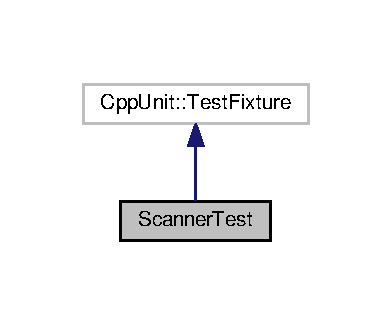
\includegraphics[width=188pt]{class_scanner_test__inherit__graph}
\end{center}
\end{figure}


Collaboration diagram for Scanner\+Test\+:\nopagebreak
\begin{figure}[H]
\begin{center}
\leavevmode
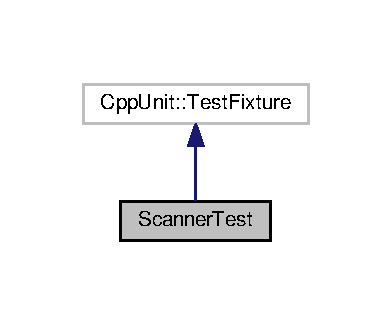
\includegraphics[width=188pt]{class_scanner_test__coll__graph}
\end{center}
\end{figure}
\subsection*{Public Member Functions}
\begin{DoxyCompactItemize}
\item 
\hyperlink{class_scanner_test_afc2605e8ad9a35e149bc51a13cba3295}{Scanner\+Test} ()
\item 
virtual \hyperlink{class_scanner_test_a3082717ef197a913610879ef283dc6d4}{$\sim$\+Scanner\+Test} ()
\item 
void \hyperlink{class_scanner_test_af1f15a7f621e57f485d905c912ff4669}{set\+Up} ()
\item 
void \hyperlink{class_scanner_test_a72e53c25dffb1a798a76c3076c1126de}{tear\+Down} ()
\end{DoxyCompactItemize}
\subsection*{Static Public Member Functions}
\begin{DoxyCompactItemize}
\item 
static Cpp\+Unit\+::\+Test $\ast$ \hyperlink{class_scanner_test_af8efe3db36a5636261c2ff60d5f13806}{suite} ()
\end{DoxyCompactItemize}
\subsection*{Protected Member Functions}
\begin{DoxyCompactItemize}
\item 
void \hyperlink{class_scanner_test_aa322e116bb9ea87b9de421b4b48541ed}{test\+Source\+File} ()
\item 
void \hyperlink{class_scanner_test_aefc9257a6d9d9f77bf6d9d67eec8fb48}{test\+Scan\+Token} ()
\end{DoxyCompactItemize}


\subsection{Constructor \& Destructor Documentation}
\index{Scanner\+Test@{Scanner\+Test}!Scanner\+Test@{Scanner\+Test}}
\index{Scanner\+Test@{Scanner\+Test}!Scanner\+Test@{Scanner\+Test}}
\subsubsection[{\texorpdfstring{Scanner\+Test()}{ScannerTest()}}]{\setlength{\rightskip}{0pt plus 5cm}Scanner\+Test\+::\+Scanner\+Test (
\begin{DoxyParamCaption}
{}
\end{DoxyParamCaption}
)}\hypertarget{class_scanner_test_afc2605e8ad9a35e149bc51a13cba3295}{}\label{class_scanner_test_afc2605e8ad9a35e149bc51a13cba3295}
\index{Scanner\+Test@{Scanner\+Test}!````~Scanner\+Test@{$\sim$\+Scanner\+Test}}
\index{````~Scanner\+Test@{$\sim$\+Scanner\+Test}!Scanner\+Test@{Scanner\+Test}}
\subsubsection[{\texorpdfstring{$\sim$\+Scanner\+Test()}{~ScannerTest()}}]{\setlength{\rightskip}{0pt plus 5cm}Scanner\+Test\+::$\sim$\+Scanner\+Test (
\begin{DoxyParamCaption}
{}
\end{DoxyParamCaption}
)\hspace{0.3cm}{\ttfamily [virtual]}}\hypertarget{class_scanner_test_a3082717ef197a913610879ef283dc6d4}{}\label{class_scanner_test_a3082717ef197a913610879ef283dc6d4}


\subsection{Member Function Documentation}
\index{Scanner\+Test@{Scanner\+Test}!set\+Up@{set\+Up}}
\index{set\+Up@{set\+Up}!Scanner\+Test@{Scanner\+Test}}
\subsubsection[{\texorpdfstring{set\+Up()}{setUp()}}]{\setlength{\rightskip}{0pt plus 5cm}void Scanner\+Test\+::set\+Up (
\begin{DoxyParamCaption}
{}
\end{DoxyParamCaption}
)}\hypertarget{class_scanner_test_af1f15a7f621e57f485d905c912ff4669}{}\label{class_scanner_test_af1f15a7f621e57f485d905c912ff4669}
\index{Scanner\+Test@{Scanner\+Test}!suite@{suite}}
\index{suite@{suite}!Scanner\+Test@{Scanner\+Test}}
\subsubsection[{\texorpdfstring{suite()}{suite()}}]{\setlength{\rightskip}{0pt plus 5cm}static Cpp\+Unit\+::\+Test$\ast$ Scanner\+Test\+::suite (
\begin{DoxyParamCaption}
{}
\end{DoxyParamCaption}
)\hspace{0.3cm}{\ttfamily [inline]}, {\ttfamily [static]}}\hypertarget{class_scanner_test_af8efe3db36a5636261c2ff60d5f13806}{}\label{class_scanner_test_af8efe3db36a5636261c2ff60d5f13806}
\index{Scanner\+Test@{Scanner\+Test}!tear\+Down@{tear\+Down}}
\index{tear\+Down@{tear\+Down}!Scanner\+Test@{Scanner\+Test}}
\subsubsection[{\texorpdfstring{tear\+Down()}{tearDown()}}]{\setlength{\rightskip}{0pt plus 5cm}void Scanner\+Test\+::tear\+Down (
\begin{DoxyParamCaption}
{}
\end{DoxyParamCaption}
)}\hypertarget{class_scanner_test_a72e53c25dffb1a798a76c3076c1126de}{}\label{class_scanner_test_a72e53c25dffb1a798a76c3076c1126de}
\index{Scanner\+Test@{Scanner\+Test}!test\+Scan\+Token@{test\+Scan\+Token}}
\index{test\+Scan\+Token@{test\+Scan\+Token}!Scanner\+Test@{Scanner\+Test}}
\subsubsection[{\texorpdfstring{test\+Scan\+Token()}{testScanToken()}}]{\setlength{\rightskip}{0pt plus 5cm}void Scanner\+Test\+::test\+Scan\+Token (
\begin{DoxyParamCaption}
{}
\end{DoxyParamCaption}
)\hspace{0.3cm}{\ttfamily [protected]}}\hypertarget{class_scanner_test_aefc9257a6d9d9f77bf6d9d67eec8fb48}{}\label{class_scanner_test_aefc9257a6d9d9f77bf6d9d67eec8fb48}
\index{Scanner\+Test@{Scanner\+Test}!test\+Source\+File@{test\+Source\+File}}
\index{test\+Source\+File@{test\+Source\+File}!Scanner\+Test@{Scanner\+Test}}
\subsubsection[{\texorpdfstring{test\+Source\+File()}{testSourceFile()}}]{\setlength{\rightskip}{0pt plus 5cm}void Scanner\+Test\+::test\+Source\+File (
\begin{DoxyParamCaption}
{}
\end{DoxyParamCaption}
)\hspace{0.3cm}{\ttfamily [protected]}}\hypertarget{class_scanner_test_aa322e116bb9ea87b9de421b4b48541ed}{}\label{class_scanner_test_aa322e116bb9ea87b9de421b4b48541ed}


The documentation for this class was generated from the following files\+:\begin{DoxyCompactItemize}
\item 
/home/vagrant/\+Projects/\+Smart\+Controller/\+Smart\+Compiler/\+Scanner\+Test/\hyperlink{_scanner_test_8h}{Scanner\+Test.\+h}\item 
/home/vagrant/\+Projects/\+Smart\+Controller/\+Smart\+Compiler/\+Scanner\+Test/\hyperlink{_scanner_test_8cpp}{Scanner\+Test.\+cpp}\end{DoxyCompactItemize}

\hypertarget{class_scanner_1_1_source_file}{}\section{Scanner\+:\+:Source\+File Class Reference}
\label{class_scanner_1_1_source_file}\index{Scanner\+::\+Source\+File@{Scanner\+::\+Source\+File}}


{\ttfamily \#include $<$Source\+File.\+h$>$}

\subsection*{Public Member Functions}
\begin{DoxyCompactItemize}
\item 
\hyperlink{class_scanner_1_1_source_file_a69413a98a0eff1311709148adfc0f222}{Source\+File} ()
\item 
virtual \hyperlink{class_scanner_1_1_source_file_a6284afa603e0dd8fbbd39ef3f3a5f6e8}{$\sim$\+Source\+File} ()
\item 
bool \hyperlink{class_scanner_1_1_source_file_a9eebbc5f778162566288961966df398c}{init} (const std\+::string \&src\+File\+Name)
\item 
int \hyperlink{class_scanner_1_1_source_file_a919d7efa693790e75e7051fc67479e34}{get\+Line\+Num} ()
\item 
int \hyperlink{class_scanner_1_1_source_file_a3e0efd4171c7225474bf1d9c5f5a8299}{get\+Col\+Num} ()
\item 
char \hyperlink{class_scanner_1_1_source_file_ac6f02448138ec25c4e8e338d645ea256}{peek\+Char} ()
\item 
char \hyperlink{class_scanner_1_1_source_file_a7592182b0200b3f095ad6642ce2f6092}{next\+Char} ()
\item 
char \hyperlink{class_scanner_1_1_source_file_a5ef11af7fec78f07581a071d631dd64d}{cur\+Char} ()
\end{DoxyCompactItemize}


\subsection{Constructor \& Destructor Documentation}
\index{Scanner\+::\+Source\+File@{Scanner\+::\+Source\+File}!Source\+File@{Source\+File}}
\index{Source\+File@{Source\+File}!Scanner\+::\+Source\+File@{Scanner\+::\+Source\+File}}
\subsubsection[{\texorpdfstring{Source\+File()}{SourceFile()}}]{\setlength{\rightskip}{0pt plus 5cm}Scanner\+::\+Source\+File\+::\+Source\+File (
\begin{DoxyParamCaption}
{}
\end{DoxyParamCaption}
)}\hypertarget{class_scanner_1_1_source_file_a69413a98a0eff1311709148adfc0f222}{}\label{class_scanner_1_1_source_file_a69413a98a0eff1311709148adfc0f222}
\index{Scanner\+::\+Source\+File@{Scanner\+::\+Source\+File}!````~Source\+File@{$\sim$\+Source\+File}}
\index{````~Source\+File@{$\sim$\+Source\+File}!Scanner\+::\+Source\+File@{Scanner\+::\+Source\+File}}
\subsubsection[{\texorpdfstring{$\sim$\+Source\+File()}{~SourceFile()}}]{\setlength{\rightskip}{0pt plus 5cm}Scanner\+::\+Source\+File\+::$\sim$\+Source\+File (
\begin{DoxyParamCaption}
{}
\end{DoxyParamCaption}
)\hspace{0.3cm}{\ttfamily [virtual]}}\hypertarget{class_scanner_1_1_source_file_a6284afa603e0dd8fbbd39ef3f3a5f6e8}{}\label{class_scanner_1_1_source_file_a6284afa603e0dd8fbbd39ef3f3a5f6e8}


\subsection{Member Function Documentation}
\index{Scanner\+::\+Source\+File@{Scanner\+::\+Source\+File}!cur\+Char@{cur\+Char}}
\index{cur\+Char@{cur\+Char}!Scanner\+::\+Source\+File@{Scanner\+::\+Source\+File}}
\subsubsection[{\texorpdfstring{cur\+Char()}{curChar()}}]{\setlength{\rightskip}{0pt plus 5cm}char Scanner\+::\+Source\+File\+::cur\+Char (
\begin{DoxyParamCaption}
{}
\end{DoxyParamCaption}
)}\hypertarget{class_scanner_1_1_source_file_a5ef11af7fec78f07581a071d631dd64d}{}\label{class_scanner_1_1_source_file_a5ef11af7fec78f07581a071d631dd64d}
\index{Scanner\+::\+Source\+File@{Scanner\+::\+Source\+File}!get\+Col\+Num@{get\+Col\+Num}}
\index{get\+Col\+Num@{get\+Col\+Num}!Scanner\+::\+Source\+File@{Scanner\+::\+Source\+File}}
\subsubsection[{\texorpdfstring{get\+Col\+Num()}{getColNum()}}]{\setlength{\rightskip}{0pt plus 5cm}int Scanner\+::\+Source\+File\+::get\+Col\+Num (
\begin{DoxyParamCaption}
{}
\end{DoxyParamCaption}
)\hspace{0.3cm}{\ttfamily [inline]}}\hypertarget{class_scanner_1_1_source_file_a3e0efd4171c7225474bf1d9c5f5a8299}{}\label{class_scanner_1_1_source_file_a3e0efd4171c7225474bf1d9c5f5a8299}
\index{Scanner\+::\+Source\+File@{Scanner\+::\+Source\+File}!get\+Line\+Num@{get\+Line\+Num}}
\index{get\+Line\+Num@{get\+Line\+Num}!Scanner\+::\+Source\+File@{Scanner\+::\+Source\+File}}
\subsubsection[{\texorpdfstring{get\+Line\+Num()}{getLineNum()}}]{\setlength{\rightskip}{0pt plus 5cm}int Scanner\+::\+Source\+File\+::get\+Line\+Num (
\begin{DoxyParamCaption}
{}
\end{DoxyParamCaption}
)\hspace{0.3cm}{\ttfamily [inline]}}\hypertarget{class_scanner_1_1_source_file_a919d7efa693790e75e7051fc67479e34}{}\label{class_scanner_1_1_source_file_a919d7efa693790e75e7051fc67479e34}
\index{Scanner\+::\+Source\+File@{Scanner\+::\+Source\+File}!init@{init}}
\index{init@{init}!Scanner\+::\+Source\+File@{Scanner\+::\+Source\+File}}
\subsubsection[{\texorpdfstring{init(const std\+::string \&src\+File\+Name)}{init(const std::string &srcFileName)}}]{\setlength{\rightskip}{0pt plus 5cm}bool Scanner\+::\+Source\+File\+::init (
\begin{DoxyParamCaption}
\item[{const std\+::string \&}]{src\+File\+Name}
\end{DoxyParamCaption}
)}\hypertarget{class_scanner_1_1_source_file_a9eebbc5f778162566288961966df398c}{}\label{class_scanner_1_1_source_file_a9eebbc5f778162566288961966df398c}
\index{Scanner\+::\+Source\+File@{Scanner\+::\+Source\+File}!next\+Char@{next\+Char}}
\index{next\+Char@{next\+Char}!Scanner\+::\+Source\+File@{Scanner\+::\+Source\+File}}
\subsubsection[{\texorpdfstring{next\+Char()}{nextChar()}}]{\setlength{\rightskip}{0pt plus 5cm}char Scanner\+::\+Source\+File\+::next\+Char (
\begin{DoxyParamCaption}
{}
\end{DoxyParamCaption}
)}\hypertarget{class_scanner_1_1_source_file_a7592182b0200b3f095ad6642ce2f6092}{}\label{class_scanner_1_1_source_file_a7592182b0200b3f095ad6642ce2f6092}
\index{Scanner\+::\+Source\+File@{Scanner\+::\+Source\+File}!peek\+Char@{peek\+Char}}
\index{peek\+Char@{peek\+Char}!Scanner\+::\+Source\+File@{Scanner\+::\+Source\+File}}
\subsubsection[{\texorpdfstring{peek\+Char()}{peekChar()}}]{\setlength{\rightskip}{0pt plus 5cm}char Scanner\+::\+Source\+File\+::peek\+Char (
\begin{DoxyParamCaption}
{}
\end{DoxyParamCaption}
)}\hypertarget{class_scanner_1_1_source_file_ac6f02448138ec25c4e8e338d645ea256}{}\label{class_scanner_1_1_source_file_ac6f02448138ec25c4e8e338d645ea256}


The documentation for this class was generated from the following files\+:\begin{DoxyCompactItemize}
\item 
/home/vagrant/\+Projects/\+Smart\+Controller/\+Smart\+Compiler/\+Scanner/\hyperlink{_source_file_8h}{Source\+File.\+h}\item 
/home/vagrant/\+Projects/\+Smart\+Controller/\+Smart\+Compiler/\+Scanner/\hyperlink{_source_file_8cpp}{Source\+File.\+cpp}\end{DoxyCompactItemize}

\hypertarget{class_scanner_1_1_token}{}\section{Scanner\+:\+:Token Class Reference}
\label{class_scanner_1_1_token}\index{Scanner\+::\+Token@{Scanner\+::\+Token}}


Inheritance diagram for Scanner\+:\+:Token\+:
\nopagebreak
\begin{figure}[H]
\begin{center}
\leavevmode
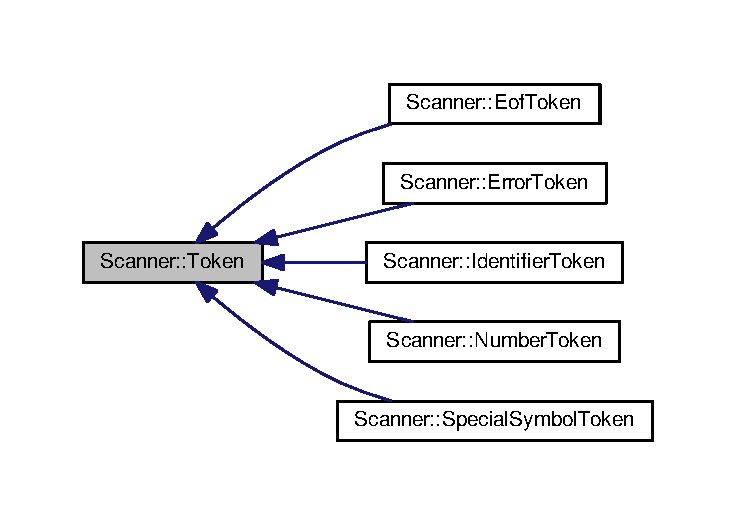
\includegraphics[width=350pt]{class_scanner_1_1_token__inherit__graph}
\end{center}
\end{figure}
\subsection*{Public Types}
\begin{DoxyCompactItemize}
\item 
enum {\bfseries E\+Token\+Type} \+: uint \{ \\*
{\bfseries E\+R\+R\+OR} = 0, 
{\bfseries E\+N\+D\+\_\+\+O\+F\+\_\+\+F\+I\+LE}, 
{\bfseries I\+D\+E\+N\+T\+I\+F\+I\+ER}, 
{\bfseries P\+R\+O\+G\+R\+AM}, 
\\*
{\bfseries E\+N\+D\+\_\+\+P\+R\+O\+G\+R\+AM}, 
{\bfseries V\+AR}, 
{\bfseries E\+N\+D\+\_\+\+V\+AR}, 
{\bfseries C\+O\+L\+O\+N\+\_\+\+S\+YM}, 
\\*
{\bfseries A\+S\+S\+I\+G\+N\+\_\+\+S\+YM}, 
{\bfseries S\+E\+M\+I\+C\+O\+L\+\_\+\+S\+YM}, 
{\bfseries P\+E\+R\+C\+E\+N\+T\+\_\+\+S\+YM}, 
{\bfseries P\+E\+R\+I\+O\+D\+\_\+\+S\+YM}, 
\\*
{\bfseries U\+N\+K\+N\+O\+WN}
 \}\hypertarget{class_scanner_1_1_token_adba36ae34c8f4befddcbc76c761cc244}{}\label{class_scanner_1_1_token_adba36ae34c8f4befddcbc76c761cc244}

\end{DoxyCompactItemize}
\subsection*{Public Member Functions}
\begin{DoxyCompactItemize}
\item 
virtual void {\bfseries scan\+Token} (\hyperlink{class_scanner_1_1_source_file}{Source\+File} \&r\+File)\hypertarget{class_scanner_1_1_token_a8a05ceeb54beba7a7212564b4f164446}{}\label{class_scanner_1_1_token_a8a05ceeb54beba7a7212564b4f164446}

\item 
E\+Token\+Type {\bfseries get\+Type} ()\hypertarget{class_scanner_1_1_token_ab1b8fca3f87cdb8d94d689bea15c9ad6}{}\label{class_scanner_1_1_token_ab1b8fca3f87cdb8d94d689bea15c9ad6}

\item 
std\+::string {\bfseries get\+Text} ()\hypertarget{class_scanner_1_1_token_a2154667730517a87309c8ca9e81552e3}{}\label{class_scanner_1_1_token_a2154667730517a87309c8ca9e81552e3}

\item 
int {\bfseries get\+Line} ()\hypertarget{class_scanner_1_1_token_a8da596b64a487ea98244ae269cda90d3}{}\label{class_scanner_1_1_token_a8da596b64a487ea98244ae269cda90d3}

\item 
int {\bfseries get\+Col} ()\hypertarget{class_scanner_1_1_token_a55e7d1b5e89057371ac3924b9cd3708b}{}\label{class_scanner_1_1_token_a55e7d1b5e89057371ac3924b9cd3708b}

\end{DoxyCompactItemize}
\subsection*{Static Public Member Functions}
\begin{DoxyCompactItemize}
\item 
static E\+Token\+Type {\bfseries text2\+Type} (const std\+::string \&some\+Text)\hypertarget{class_scanner_1_1_token_a9d998150939f8ef7fcd0a50f6bece5d8}{}\label{class_scanner_1_1_token_a9d998150939f8ef7fcd0a50f6bece5d8}

\item 
static bool {\bfseries is\+Key\+Word} (const std\+::string \&some\+Text)\hypertarget{class_scanner_1_1_token_a76634cafc7a564d36533376a8ee58f58}{}\label{class_scanner_1_1_token_a76634cafc7a564d36533376a8ee58f58}

\item 
static bool {\bfseries is\+Special\+Symbol} (const std\+::string \&some\+Text)\hypertarget{class_scanner_1_1_token_adc64dc5bb8e26e9b238ac940395826f3}{}\label{class_scanner_1_1_token_adc64dc5bb8e26e9b238ac940395826f3}

\end{DoxyCompactItemize}
\subsection*{Static Public Attributes}
\begin{DoxyCompactItemize}
\item 
static const std\+::vector$<$ std\+::string $>$ {\bfseries Token\+Text}
\item 
static const std\+::vector$<$ E\+Token\+Type $>$ {\bfseries Key\+Words}
\item 
static const std\+::vector$<$ E\+Token\+Type $>$ {\bfseries Special\+Symbols}
\end{DoxyCompactItemize}
\subsection*{Protected Attributes}
\begin{DoxyCompactItemize}
\item 
E\+Token\+Type {\bfseries m\+\_\+token\+Type}\hypertarget{class_scanner_1_1_token_afdb4cd3121e353221f190997dd20648f}{}\label{class_scanner_1_1_token_afdb4cd3121e353221f190997dd20648f}

\item 
std\+::string {\bfseries m\+\_\+token\+Text}\hypertarget{class_scanner_1_1_token_a03cda26b93d4751fe631c65912e6d446}{}\label{class_scanner_1_1_token_a03cda26b93d4751fe631c65912e6d446}

\item 
int {\bfseries m\+\_\+line\+Num}\hypertarget{class_scanner_1_1_token_a00d8f8fc6715651a1a02e11579ce099f}{}\label{class_scanner_1_1_token_a00d8f8fc6715651a1a02e11579ce099f}

\item 
int {\bfseries m\+\_\+col\+Num}\hypertarget{class_scanner_1_1_token_a34c62ba179be0a9881fe5fb0c38f89b1}{}\label{class_scanner_1_1_token_a34c62ba179be0a9881fe5fb0c38f89b1}

\end{DoxyCompactItemize}


\subsection{Member Data Documentation}
\index{Scanner\+::\+Token@{Scanner\+::\+Token}!Key\+Words@{Key\+Words}}
\index{Key\+Words@{Key\+Words}!Scanner\+::\+Token@{Scanner\+::\+Token}}
\subsubsection[{\texorpdfstring{Key\+Words}{KeyWords}}]{\setlength{\rightskip}{0pt plus 5cm}const std\+::vector$<$ Token\+::\+E\+Token\+Type $>$ Scanner\+::\+Token\+::\+Key\+Words\hspace{0.3cm}{\ttfamily [static]}}\hypertarget{class_scanner_1_1_token_ac3bfa7f186802c0fac1dbbcc379b4978}{}\label{class_scanner_1_1_token_ac3bfa7f186802c0fac1dbbcc379b4978}
{\bfseries Initial value\+:}
\begin{DoxyCode}
=
\{
    ETokenType::PROGRAM,
    ETokenType::END\_PROGRAM,
    ETokenType::VAR,
    ETokenType::END\_VAR,
\}
\end{DoxyCode}
\index{Scanner\+::\+Token@{Scanner\+::\+Token}!Special\+Symbols@{Special\+Symbols}}
\index{Special\+Symbols@{Special\+Symbols}!Scanner\+::\+Token@{Scanner\+::\+Token}}
\subsubsection[{\texorpdfstring{Special\+Symbols}{SpecialSymbols}}]{\setlength{\rightskip}{0pt plus 5cm}const std\+::vector$<$ Token\+::\+E\+Token\+Type $>$ Scanner\+::\+Token\+::\+Special\+Symbols\hspace{0.3cm}{\ttfamily [static]}}\hypertarget{class_scanner_1_1_token_a717646234da005d9ccb185c1f782afd1}{}\label{class_scanner_1_1_token_a717646234da005d9ccb185c1f782afd1}
{\bfseries Initial value\+:}
\begin{DoxyCode}
=
\{
    ETokenType::COLON\_SYM,
    ETokenType::ASSIGN\_SYM,
    ETokenType::SEMICOL\_SYM,
    ETokenType::PERCENT\_SYM,
    ETokenType::PERIOD\_SYM,
\}
\end{DoxyCode}
\index{Scanner\+::\+Token@{Scanner\+::\+Token}!Token\+Text@{Token\+Text}}
\index{Token\+Text@{Token\+Text}!Scanner\+::\+Token@{Scanner\+::\+Token}}
\subsubsection[{\texorpdfstring{Token\+Text}{TokenText}}]{\setlength{\rightskip}{0pt plus 5cm}const std\+::vector$<$ std\+::string $>$ Scanner\+::\+Token\+::\+Token\+Text\hspace{0.3cm}{\ttfamily [static]}}\hypertarget{class_scanner_1_1_token_a01fb9e95d9a1c93f3e6adf3ea208bf36}{}\label{class_scanner_1_1_token_a01fb9e95d9a1c93f3e6adf3ea208bf36}
{\bfseries Initial value\+:}
\begin{DoxyCode}
=
\{
    \textcolor{stringliteral}{"ERROR"},
    \textcolor{stringliteral}{"END\_OF\_FILE"},
    \textcolor{stringliteral}{"IDENTIFIER"},
    \textcolor{stringliteral}{"PROGRAM"},
    \textcolor{stringliteral}{"END\_PROGRAM"},
    \textcolor{stringliteral}{"VAR"},
    \textcolor{stringliteral}{"END\_VAR"},
    \textcolor{stringliteral}{":"},
    \textcolor{stringliteral}{":="},
    \textcolor{stringliteral}{";"},
    \textcolor{stringliteral}{"%"},
    \textcolor{stringliteral}{"."},
    \textcolor{stringliteral}{"UNKNOWN"},
\}
\end{DoxyCode}


The documentation for this class was generated from the following files\+:\begin{DoxyCompactItemize}
\item 
Scanner/Token.\+h\item 
Scanner/Token.\+cpp\end{DoxyCompactItemize}

\hypertarget{class_util_1_1_util_test}{}\section{Util\+:\+:Util\+Test Class Reference}
\label{class_util_1_1_util_test}\index{Util\+::\+Util\+Test@{Util\+::\+Util\+Test}}


Inheritance diagram for Util\+:\+:Util\+Test\+:
\nopagebreak
\begin{figure}[H]
\begin{center}
\leavevmode
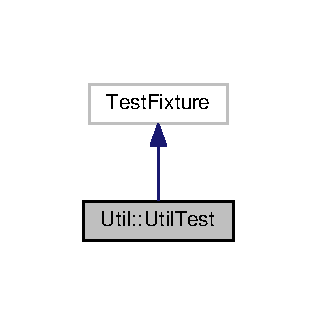
\includegraphics[width=152pt]{class_util_1_1_util_test__inherit__graph}
\end{center}
\end{figure}


Collaboration diagram for Util\+:\+:Util\+Test\+:
\nopagebreak
\begin{figure}[H]
\begin{center}
\leavevmode
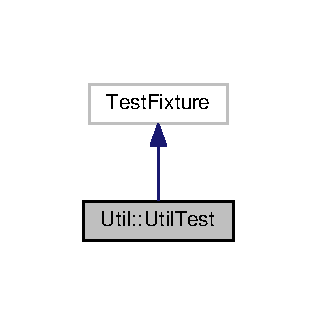
\includegraphics[width=152pt]{class_util_1_1_util_test__coll__graph}
\end{center}
\end{figure}
\subsection*{Public Member Functions}
\begin{DoxyCompactItemize}
\item 
void {\bfseries set\+Up} ()\hypertarget{class_util_1_1_util_test_a10968ee4258f61df4caa1dbba822b9e6}{}\label{class_util_1_1_util_test_a10968ee4258f61df4caa1dbba822b9e6}

\item 
void {\bfseries tear\+Down} ()\hypertarget{class_util_1_1_util_test_a0b0e3dd728dc81fc516b35ed14f7ab7e}{}\label{class_util_1_1_util_test_a0b0e3dd728dc81fc516b35ed14f7ab7e}

\end{DoxyCompactItemize}
\subsection*{Static Public Member Functions}
\begin{DoxyCompactItemize}
\item 
static Cpp\+Unit\+::\+Test $\ast$ {\bfseries suite} ()\hypertarget{class_util_1_1_util_test_a6aea16da6a30f2da7c331884402678e9}{}\label{class_util_1_1_util_test_a6aea16da6a30f2da7c331884402678e9}

\end{DoxyCompactItemize}
\subsection*{Protected Member Functions}
\begin{DoxyCompactItemize}
\item 
void {\bfseries test\+Time} ()\hypertarget{class_util_1_1_util_test_a6df1223c040166a5e42610f6ceb76666}{}\label{class_util_1_1_util_test_a6df1223c040166a5e42610f6ceb76666}

\item 
void {\bfseries test\+Message\+Mgr} ()\hypertarget{class_util_1_1_util_test_a3e88702de7b7d45377b1dc99f22bbc3a}{}\label{class_util_1_1_util_test_a3e88702de7b7d45377b1dc99f22bbc3a}

\item 
void {\bfseries test\+Config\+Reader} ()\hypertarget{class_util_1_1_util_test_ae46a726defc5ffe24f126ca1d7da3775}{}\label{class_util_1_1_util_test_ae46a726defc5ffe24f126ca1d7da3775}

\end{DoxyCompactItemize}


The documentation for this class was generated from the following files\+:\begin{DoxyCompactItemize}
\item 
Util\+Test/Util\+Test.\+h\item 
Util\+Test/Util\+Test.\+cpp\end{DoxyCompactItemize}

\chapter{File Documentation}
\hypertarget{setup_8dox}{}\section{setup.\+dox File Reference}
\label{setup_8dox}\index{setup.\+dox@{setup.\+dox}}

\hypertarget{_scanner_s_t_8d}{}\section{/home/vagrant/\+Projects/\+Smart\+Controller/\+Smart\+Compiler/\+Scanner/\+Debug/\+Scanner\+ST.d File Reference}
\label{_scanner_s_t_8d}\index{/home/vagrant/\+Projects/\+Smart\+Controller/\+Smart\+Compiler/\+Scanner/\+Debug/\+Scanner\+S\+T.\+d@{/home/vagrant/\+Projects/\+Smart\+Controller/\+Smart\+Compiler/\+Scanner/\+Debug/\+Scanner\+S\+T.\+d}}

\hypertarget{_source_file_8d}{}\section{/home/vagrant/\+Projects/\+Smart\+Controller/\+Smart\+Compiler/\+Scanner/\+Debug/\+Source\+File.d File Reference}
\label{_source_file_8d}\index{/home/vagrant/\+Projects/\+Smart\+Controller/\+Smart\+Compiler/\+Scanner/\+Debug/\+Source\+File.\+d@{/home/vagrant/\+Projects/\+Smart\+Controller/\+Smart\+Compiler/\+Scanner/\+Debug/\+Source\+File.\+d}}

\hypertarget{_token_8d}{}\section{/home/vagrant/\+Projects/\+Smart\+Controller/\+Smart\+Compiler/\+Scanner/\+Debug/\+Token.d File Reference}
\label{_token_8d}\index{/home/vagrant/\+Projects/\+Smart\+Controller/\+Smart\+Compiler/\+Scanner/\+Debug/\+Token.\+d@{/home/vagrant/\+Projects/\+Smart\+Controller/\+Smart\+Compiler/\+Scanner/\+Debug/\+Token.\+d}}

\hypertarget{_scanner_s_t_8cpp}{}\section{/home/vagrant/\+Projects/\+Smart\+Controller/\+Smart\+Compiler/\+Scanner/\+Scanner\+ST.cpp File Reference}
\label{_scanner_s_t_8cpp}\index{/home/vagrant/\+Projects/\+Smart\+Controller/\+Smart\+Compiler/\+Scanner/\+Scanner\+S\+T.\+cpp@{/home/vagrant/\+Projects/\+Smart\+Controller/\+Smart\+Compiler/\+Scanner/\+Scanner\+S\+T.\+cpp}}
{\ttfamily \#include $<$stdio.\+h$>$}\\*
{\ttfamily \#include $<$memory$>$}\\*
{\ttfamily \#include \char`\"{}Token.\+h\char`\"{}}\\*
{\ttfamily \#include \char`\"{}Source\+File.\+h\char`\"{}}\\*
{\ttfamily \#include \char`\"{}Scanner\+S\+T.\+h\char`\"{}}\\*
Include dependency graph for Scanner\+S\+T.\+cpp\+:\nopagebreak
\begin{figure}[H]
\begin{center}
\leavevmode
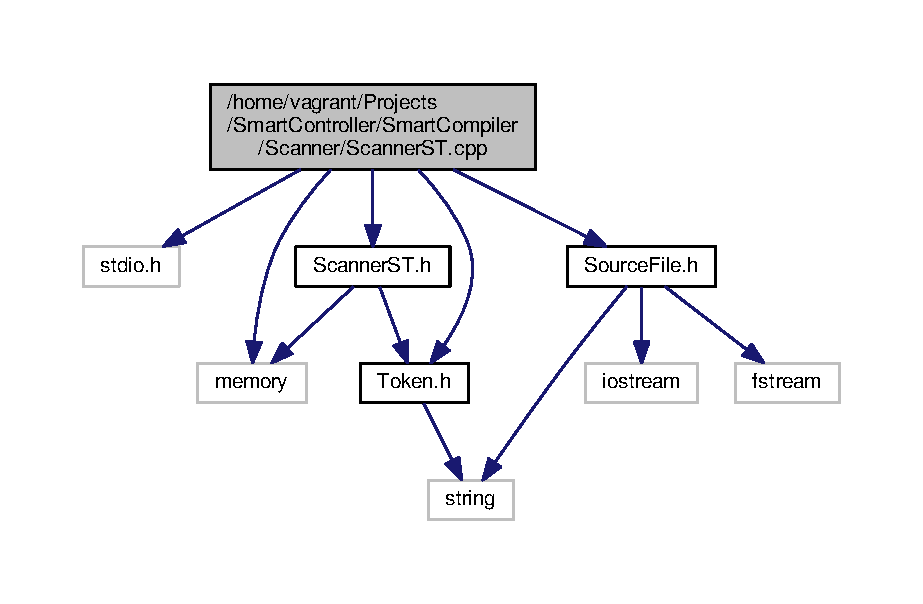
\includegraphics[width=350pt]{_scanner_s_t_8cpp__incl}
\end{center}
\end{figure}
\subsection*{Namespaces}
\begin{DoxyCompactItemize}
\item 
 \hyperlink{namespace_scanner}{Scanner}
\end{DoxyCompactItemize}

\hypertarget{_scanner_s_t_8h}{}\section{/home/vagrant/\+Projects/\+Smart\+Controller/\+Smart\+Compiler/\+Scanner/\+Scanner\+ST.h File Reference}
\label{_scanner_s_t_8h}\index{/home/vagrant/\+Projects/\+Smart\+Controller/\+Smart\+Compiler/\+Scanner/\+Scanner\+S\+T.\+h@{/home/vagrant/\+Projects/\+Smart\+Controller/\+Smart\+Compiler/\+Scanner/\+Scanner\+S\+T.\+h}}
{\ttfamily \#include $<$memory$>$}\\*
{\ttfamily \#include \char`\"{}Token.\+h\char`\"{}}\\*
Include dependency graph for Scanner\+S\+T.\+h\+:\nopagebreak
\begin{figure}[H]
\begin{center}
\leavevmode
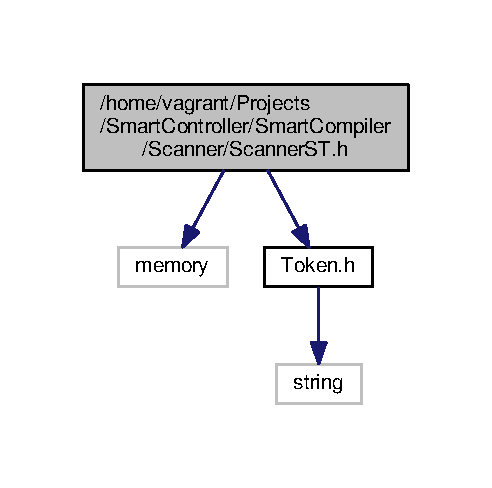
\includegraphics[width=236pt]{_scanner_s_t_8h__incl}
\end{center}
\end{figure}
This graph shows which files directly or indirectly include this file\+:\nopagebreak
\begin{figure}[H]
\begin{center}
\leavevmode
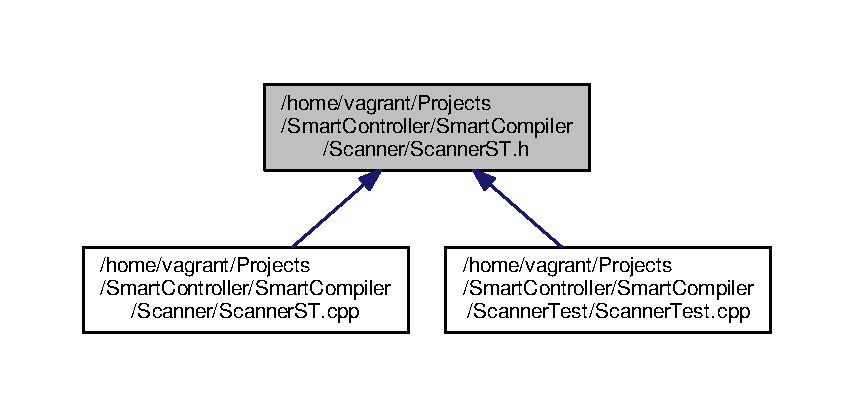
\includegraphics[width=350pt]{_scanner_s_t_8h__dep__incl}
\end{center}
\end{figure}
\subsection*{Classes}
\begin{DoxyCompactItemize}
\item 
class \hyperlink{class_scanner_1_1_scanner_s_t}{Scanner\+::\+Scanner\+ST}
\end{DoxyCompactItemize}
\subsection*{Namespaces}
\begin{DoxyCompactItemize}
\item 
 \hyperlink{namespace_scanner}{Scanner}
\end{DoxyCompactItemize}

\hypertarget{_source_file_8cpp}{}\section{/home/vagrant/\+Projects/\+Smart\+Controller/\+Smart\+Compiler/\+Scanner/\+Source\+File.cpp File Reference}
\label{_source_file_8cpp}\index{/home/vagrant/\+Projects/\+Smart\+Controller/\+Smart\+Compiler/\+Scanner/\+Source\+File.\+cpp@{/home/vagrant/\+Projects/\+Smart\+Controller/\+Smart\+Compiler/\+Scanner/\+Source\+File.\+cpp}}
{\ttfamily \#include $<$stdio.\+h$>$}\\*
{\ttfamily \#include \char`\"{}Source\+File.\+h\char`\"{}}\\*
Include dependency graph for Source\+File.\+cpp\+:\nopagebreak
\begin{figure}[H]
\begin{center}
\leavevmode
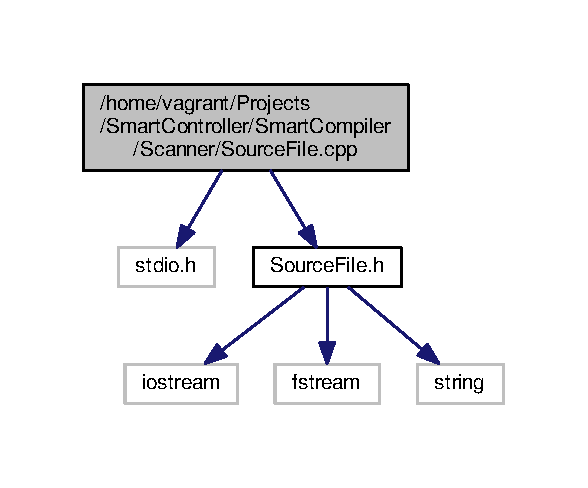
\includegraphics[width=282pt]{_source_file_8cpp__incl}
\end{center}
\end{figure}
\subsection*{Namespaces}
\begin{DoxyCompactItemize}
\item 
 \hyperlink{namespace_scanner}{Scanner}
\end{DoxyCompactItemize}

\hypertarget{_source_file_8h}{}\section{/home/vagrant/\+Projects/\+Smart\+Controller/\+Smart\+Compiler/\+Scanner/\+Source\+File.h File Reference}
\label{_source_file_8h}\index{/home/vagrant/\+Projects/\+Smart\+Controller/\+Smart\+Compiler/\+Scanner/\+Source\+File.\+h@{/home/vagrant/\+Projects/\+Smart\+Controller/\+Smart\+Compiler/\+Scanner/\+Source\+File.\+h}}
{\ttfamily \#include $<$iostream$>$}\\*
{\ttfamily \#include $<$fstream$>$}\\*
{\ttfamily \#include $<$string$>$}\\*
Include dependency graph for Source\+File.\+h\+:\nopagebreak
\begin{figure}[H]
\begin{center}
\leavevmode
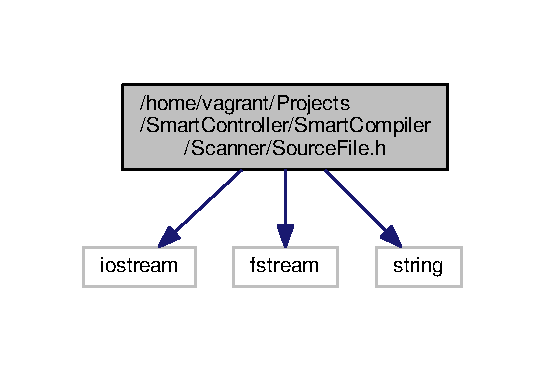
\includegraphics[width=262pt]{_source_file_8h__incl}
\end{center}
\end{figure}
This graph shows which files directly or indirectly include this file\+:\nopagebreak
\begin{figure}[H]
\begin{center}
\leavevmode
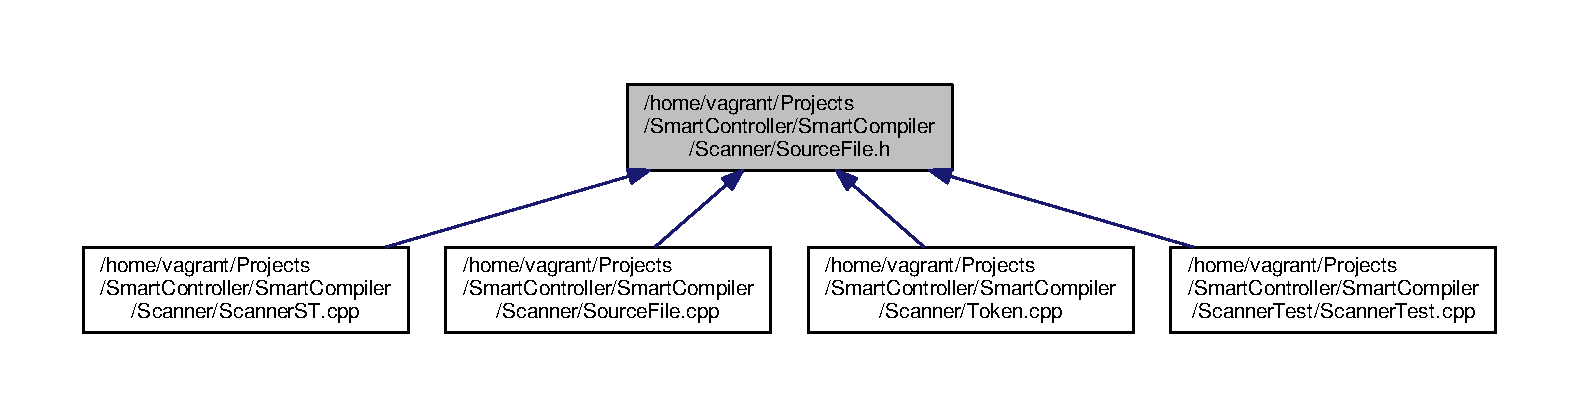
\includegraphics[width=350pt]{_source_file_8h__dep__incl}
\end{center}
\end{figure}
\subsection*{Classes}
\begin{DoxyCompactItemize}
\item 
class \hyperlink{class_scanner_1_1_source_file}{Scanner\+::\+Source\+File}
\end{DoxyCompactItemize}
\subsection*{Namespaces}
\begin{DoxyCompactItemize}
\item 
 \hyperlink{namespace_scanner}{Scanner}
\end{DoxyCompactItemize}
\subsection*{Variables}
\begin{DoxyCompactItemize}
\item 
constexpr char \hyperlink{namespace_scanner_a7859e3bfe9933aec7ee80c2d4dcfe948}{Scanner\+::\+E\+OL} \{\textquotesingle{}\textbackslash{}n\textquotesingle{}\}
\end{DoxyCompactItemize}

\hypertarget{_token_8cpp}{}\section{/home/vagrant/\+Projects/\+Smart\+Controller/\+Smart\+Compiler/\+Scanner/\+Token.cpp File Reference}
\label{_token_8cpp}\index{/home/vagrant/\+Projects/\+Smart\+Controller/\+Smart\+Compiler/\+Scanner/\+Token.\+cpp@{/home/vagrant/\+Projects/\+Smart\+Controller/\+Smart\+Compiler/\+Scanner/\+Token.\+cpp}}
{\ttfamily \#include \char`\"{}Source\+File.\+h\char`\"{}}\\*
{\ttfamily \#include \char`\"{}Token.\+h\char`\"{}}\\*
Include dependency graph for Token.\+cpp\+:\nopagebreak
\begin{figure}[H]
\begin{center}
\leavevmode
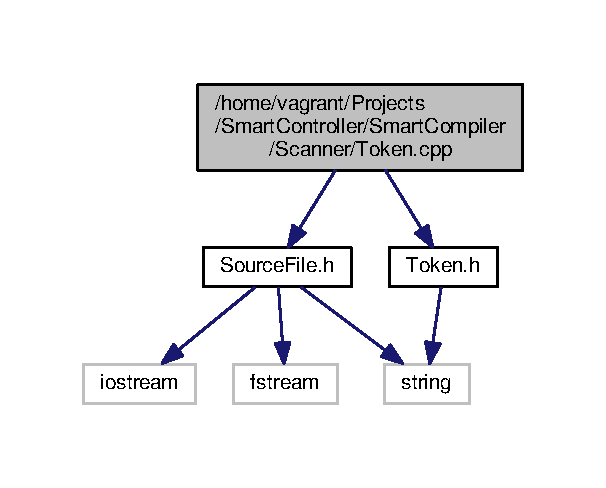
\includegraphics[width=291pt]{_token_8cpp__incl}
\end{center}
\end{figure}
\subsection*{Namespaces}
\begin{DoxyCompactItemize}
\item 
 \hyperlink{namespace_scanner}{Scanner}
\end{DoxyCompactItemize}

\hypertarget{_token_8h}{}\section{/home/vagrant/\+Projects/\+Smart\+Controller/\+Smart\+Compiler/\+Scanner/\+Token.h File Reference}
\label{_token_8h}\index{/home/vagrant/\+Projects/\+Smart\+Controller/\+Smart\+Compiler/\+Scanner/\+Token.\+h@{/home/vagrant/\+Projects/\+Smart\+Controller/\+Smart\+Compiler/\+Scanner/\+Token.\+h}}
{\ttfamily \#include $<$string$>$}\\*
Include dependency graph for Token.\+h\+:\nopagebreak
\begin{figure}[H]
\begin{center}
\leavevmode
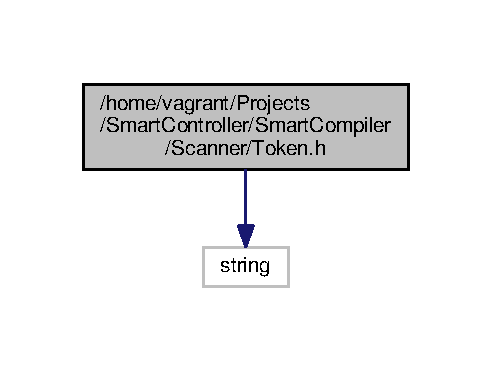
\includegraphics[width=236pt]{_token_8h__incl}
\end{center}
\end{figure}
This graph shows which files directly or indirectly include this file\+:\nopagebreak
\begin{figure}[H]
\begin{center}
\leavevmode
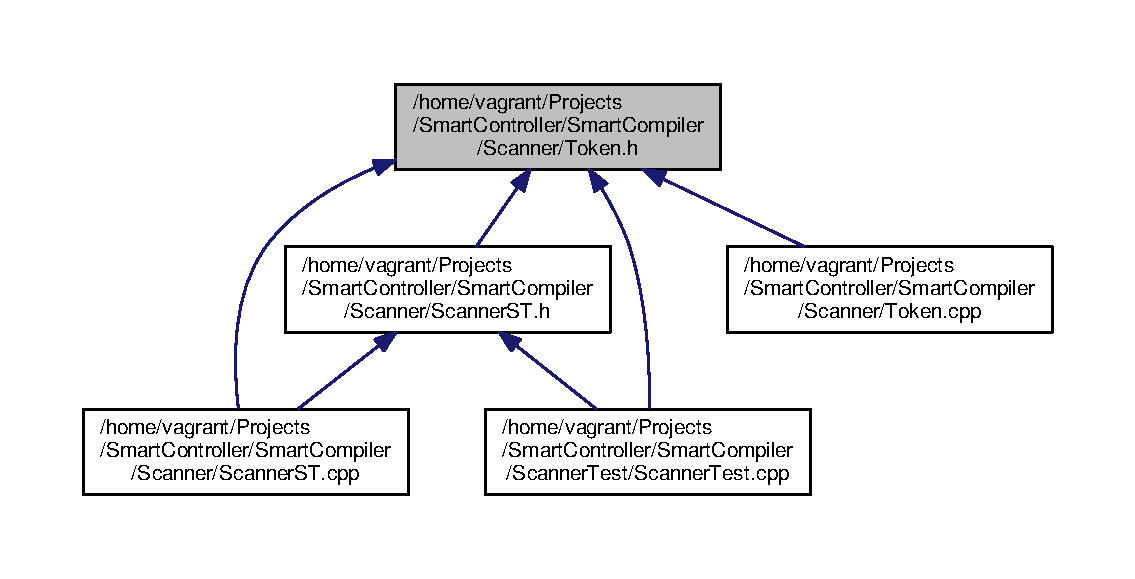
\includegraphics[width=350pt]{_token_8h__dep__incl}
\end{center}
\end{figure}
\subsection*{Classes}
\begin{DoxyCompactItemize}
\item 
class \hyperlink{class_scanner_1_1_token}{Scanner\+::\+Token}
\end{DoxyCompactItemize}
\subsection*{Namespaces}
\begin{DoxyCompactItemize}
\item 
 \hyperlink{namespace_scanner}{Scanner}
\end{DoxyCompactItemize}
\subsection*{Enumerations}
\begin{DoxyCompactItemize}
\item 
enum \hyperlink{namespace_scanner_a1d588ca5cfd26bdff0e59b437da5b166}{Scanner\+::\+Token\+Type} \{ \\*
\hyperlink{namespace_scanner_a1d588ca5cfd26bdff0e59b437da5b166a48ae1c67b152fd4cceb1fc919c07cef3}{Scanner\+::\+U\+N\+K\+N\+O\+WN}, 
\hyperlink{namespace_scanner_a1d588ca5cfd26bdff0e59b437da5b166afa7aaa30e05994a154a6659a8fc5bc0a}{Scanner\+::\+E\+R\+R\+OR}, 
\hyperlink{namespace_scanner_a1d588ca5cfd26bdff0e59b437da5b166ad9fa4b9d9c85ef41caa4540fb385491d}{Scanner\+::\+I\+D\+E\+N\+T\+I\+F\+I\+ER}, 
\hyperlink{namespace_scanner_a1d588ca5cfd26bdff0e59b437da5b166aceb64e2af79584079e0e3f3c32ccaf9d}{Scanner\+::\+P\+R\+O\+G\+R\+AM}, 
\\*
\hyperlink{namespace_scanner_a1d588ca5cfd26bdff0e59b437da5b166a32d6b00cdc94cf860b8d967cb30d7952}{Scanner\+::\+E\+N\+D\+\_\+\+P\+R\+O\+G\+R\+AM}
 \}
\end{DoxyCompactItemize}
\subsection*{Variables}
\begin{DoxyCompactItemize}
\item 
const char $\ast$const \hyperlink{namespace_scanner_a09cc779e796381e91b23d01033206d4d}{Scanner\+::\+Token\+Text} \mbox{[}$\,$\mbox{]} = \{\char`\"{}U\+N\+K\+N\+O\+WN\char`\"{}, \char`\"{}E\+R\+R\+OR\char`\"{}, \char`\"{}I\+D\+E\+N\+T\+I\+F\+I\+ER\char`\"{}, \char`\"{}P\+R\+O\+G\+R\+AM\char`\"{}, \char`\"{}E\+N\+D\+\_\+\+P\+R\+O\+G\+R\+AM\char`\"{}, \}
\item 
const char $\ast$const \hyperlink{namespace_scanner_ab32f938f9fc4150c1017a768a8843f85}{Scanner\+::\+Key\+Words} \mbox{[}$\,$\mbox{]} = \{\char`\"{}\char`\"{} , \char`\"{}\char`\"{} , \char`\"{}\char`\"{} , \char`\"{}P\+R\+O\+G\+R\+AM\char`\"{}, \char`\"{}E\+N\+D\+\_\+\+P\+R\+O\+G\+R\+AM\char`\"{}, \}
\end{DoxyCompactItemize}

\hypertarget{_scanner_test_8cpp}{}\section{/home/vagrant/\+Projects/\+Smart\+Controller/\+Smart\+Compiler/\+Scanner\+Test/\+Scanner\+Test.cpp File Reference}
\label{_scanner_test_8cpp}\index{/home/vagrant/\+Projects/\+Smart\+Controller/\+Smart\+Compiler/\+Scanner\+Test/\+Scanner\+Test.\+cpp@{/home/vagrant/\+Projects/\+Smart\+Controller/\+Smart\+Compiler/\+Scanner\+Test/\+Scanner\+Test.\+cpp}}
{\ttfamily \#include $<$stdio.\+h$>$}\\*
{\ttfamily \#include $<$memory$>$}\\*
{\ttfamily \#include \char`\"{}Logger.\+h\char`\"{}}\\*
{\ttfamily \#include \char`\"{}Token.\+h\char`\"{}}\\*
{\ttfamily \#include \char`\"{}Source\+File.\+h\char`\"{}}\\*
{\ttfamily \#include \char`\"{}Scanner\+S\+T.\+h\char`\"{}}\\*
{\ttfamily \#include \char`\"{}Scanner\+Test.\+h\char`\"{}}\\*
Include dependency graph for Scanner\+Test.\+cpp\+:\nopagebreak
\begin{figure}[H]
\begin{center}
\leavevmode
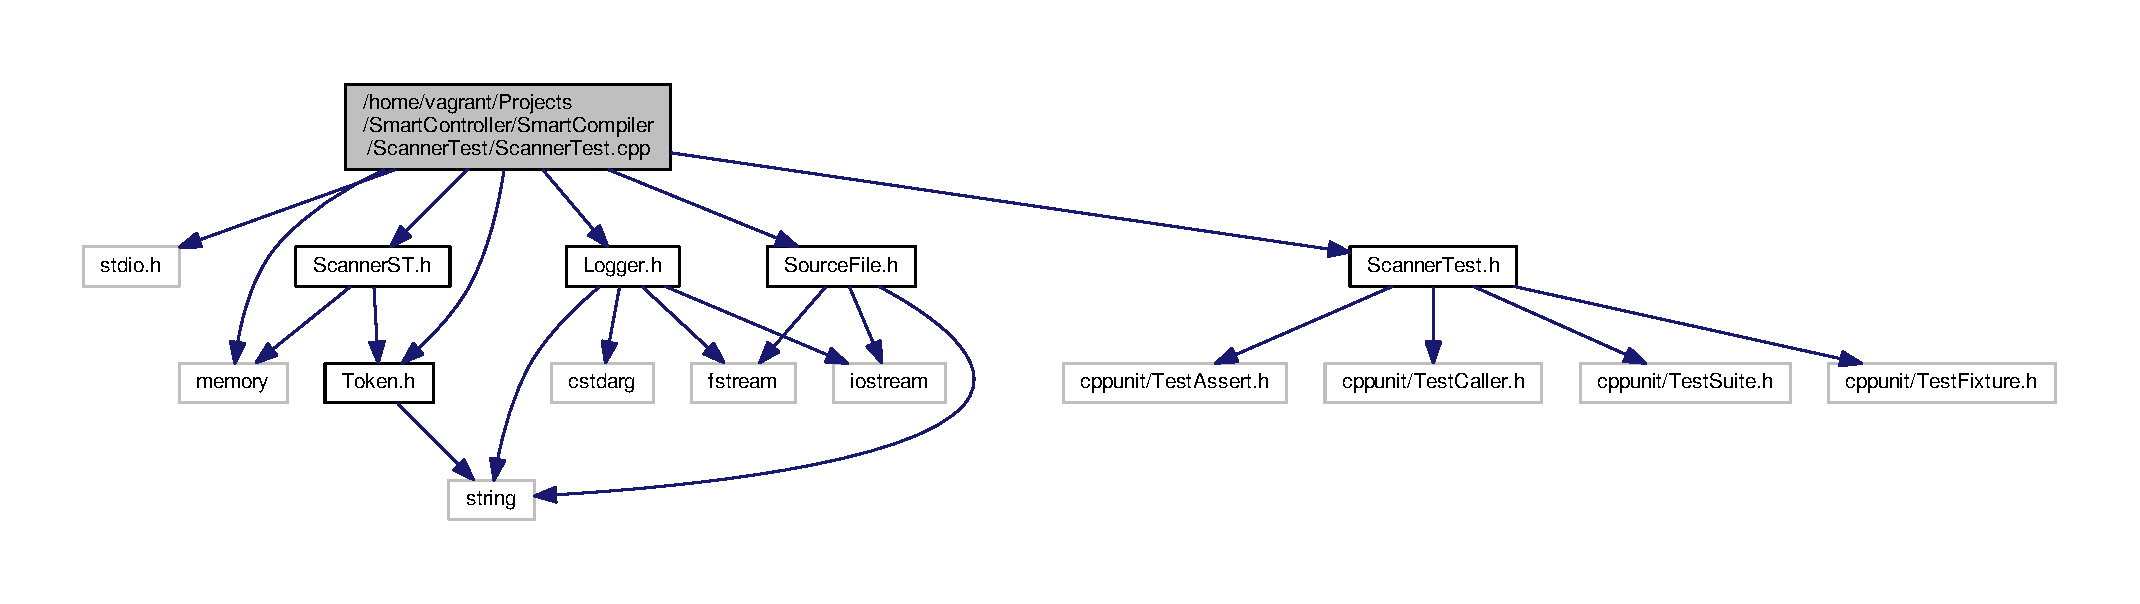
\includegraphics[width=350pt]{_scanner_test_8cpp__incl}
\end{center}
\end{figure}

\hypertarget{_scanner_test_8h}{}\section{/home/vagrant/\+Projects/\+Smart\+Controller/\+Smart\+Compiler/\+Scanner\+Test/\+Scanner\+Test.h File Reference}
\label{_scanner_test_8h}\index{/home/vagrant/\+Projects/\+Smart\+Controller/\+Smart\+Compiler/\+Scanner\+Test/\+Scanner\+Test.\+h@{/home/vagrant/\+Projects/\+Smart\+Controller/\+Smart\+Compiler/\+Scanner\+Test/\+Scanner\+Test.\+h}}
{\ttfamily \#include $<$cppunit/\+Test\+Fixture.\+h$>$}\\*
{\ttfamily \#include $<$cppunit/\+Test\+Assert.\+h$>$}\\*
{\ttfamily \#include $<$cppunit/\+Test\+Caller.\+h$>$}\\*
{\ttfamily \#include $<$cppunit/\+Test\+Suite.\+h$>$}\\*
Include dependency graph for Scanner\+Test.\+h\+:\nopagebreak
\begin{figure}[H]
\begin{center}
\leavevmode
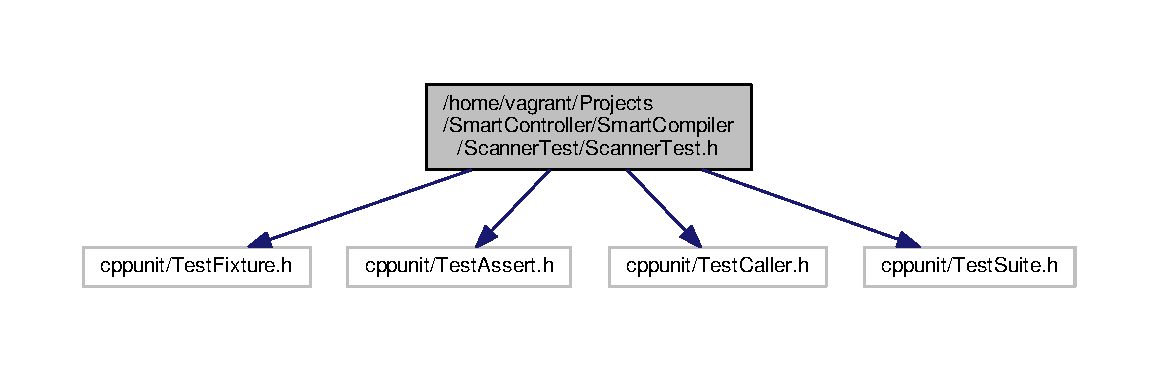
\includegraphics[width=350pt]{_scanner_test_8h__incl}
\end{center}
\end{figure}
This graph shows which files directly or indirectly include this file\+:\nopagebreak
\begin{figure}[H]
\begin{center}
\leavevmode
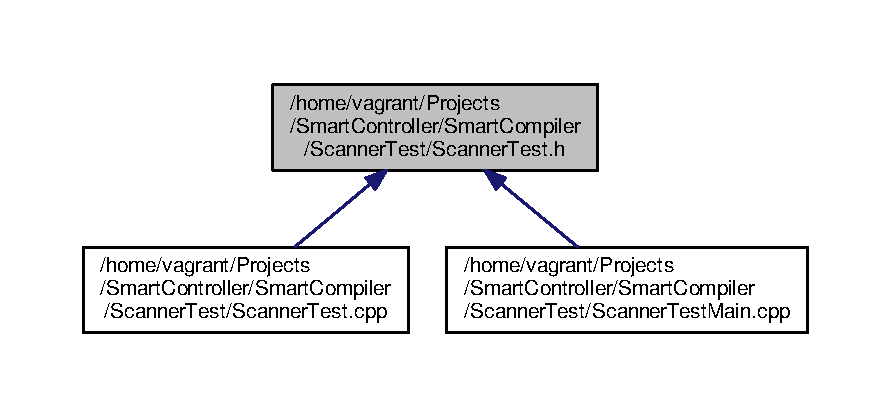
\includegraphics[width=350pt]{_scanner_test_8h__dep__incl}
\end{center}
\end{figure}
\subsection*{Classes}
\begin{DoxyCompactItemize}
\item 
class \hyperlink{class_scanner_test}{Scanner\+Test}
\end{DoxyCompactItemize}
\subsection*{Macros}
\begin{DoxyCompactItemize}
\item 
\#define \hyperlink{_scanner_test_8h_a6b20d41d6252e9871430c242cb1a56e7}{B\+U\+F\+F\+E\+R\+\_\+\+S\+I\+ZE}~1048576
\end{DoxyCompactItemize}


\subsection{Macro Definition Documentation}
\index{Scanner\+Test.\+h@{Scanner\+Test.\+h}!B\+U\+F\+F\+E\+R\+\_\+\+S\+I\+ZE@{B\+U\+F\+F\+E\+R\+\_\+\+S\+I\+ZE}}
\index{B\+U\+F\+F\+E\+R\+\_\+\+S\+I\+ZE@{B\+U\+F\+F\+E\+R\+\_\+\+S\+I\+ZE}!Scanner\+Test.\+h@{Scanner\+Test.\+h}}
\subsubsection[{\texorpdfstring{B\+U\+F\+F\+E\+R\+\_\+\+S\+I\+ZE}{BUFFER_SIZE}}]{\setlength{\rightskip}{0pt plus 5cm}\#define B\+U\+F\+F\+E\+R\+\_\+\+S\+I\+ZE~1048576}\hypertarget{_scanner_test_8h_a6b20d41d6252e9871430c242cb1a56e7}{}\label{_scanner_test_8h_a6b20d41d6252e9871430c242cb1a56e7}

\hypertarget{_scanner_test_main_8cpp}{}\section{/home/vagrant/\+Projects/\+Smart\+Controller/\+Smart\+Compiler/\+Scanner\+Test/\+Scanner\+Test\+Main.cpp File Reference}
\label{_scanner_test_main_8cpp}\index{/home/vagrant/\+Projects/\+Smart\+Controller/\+Smart\+Compiler/\+Scanner\+Test/\+Scanner\+Test\+Main.\+cpp@{/home/vagrant/\+Projects/\+Smart\+Controller/\+Smart\+Compiler/\+Scanner\+Test/\+Scanner\+Test\+Main.\+cpp}}
{\ttfamily \#include $<$iostream$>$}\\*
{\ttfamily \#include $<$cppunit/\+Test\+Suite.\+h$>$}\\*
{\ttfamily \#include $<$cppunit/ui/text/\+Test\+Runner.\+h$>$}\\*
{\ttfamily \#include \char`\"{}Scanner\+Test.\+h\char`\"{}}\\*
Include dependency graph for Scanner\+Test\+Main.\+cpp\+:\nopagebreak
\begin{figure}[H]
\begin{center}
\leavevmode
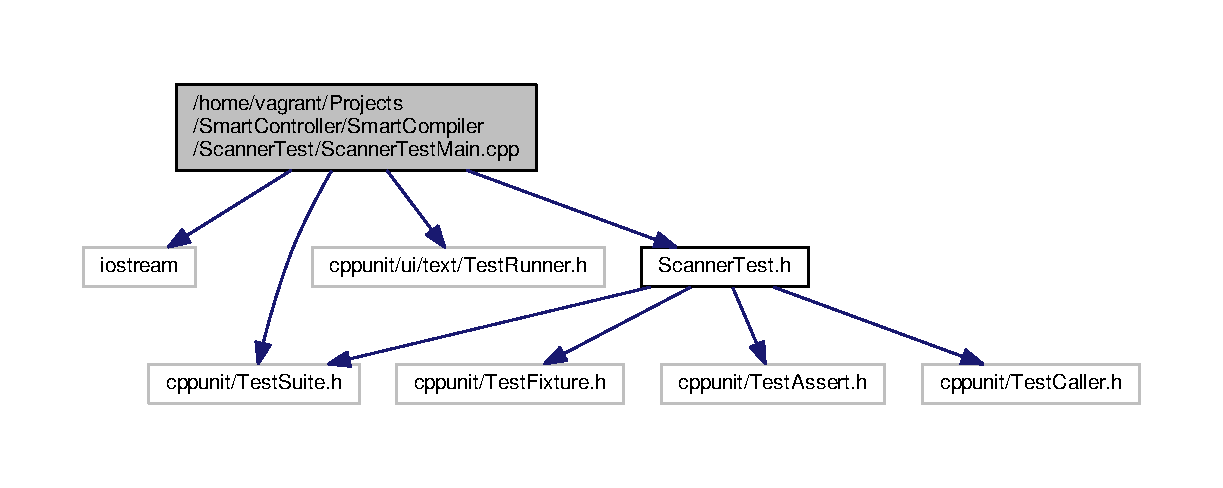
\includegraphics[width=350pt]{_scanner_test_main_8cpp__incl}
\end{center}
\end{figure}
\subsection*{Functions}
\begin{DoxyCompactItemize}
\item 
int \hyperlink{_scanner_test_main_8cpp_ae66f6b31b5ad750f1fe042a706a4e3d4}{main} ()
\end{DoxyCompactItemize}


\subsection{Function Documentation}
\index{Scanner\+Test\+Main.\+cpp@{Scanner\+Test\+Main.\+cpp}!main@{main}}
\index{main@{main}!Scanner\+Test\+Main.\+cpp@{Scanner\+Test\+Main.\+cpp}}
\subsubsection[{\texorpdfstring{main()}{main()}}]{\setlength{\rightskip}{0pt plus 5cm}int main (
\begin{DoxyParamCaption}
{}
\end{DoxyParamCaption}
)}\hypertarget{_scanner_test_main_8cpp_ae66f6b31b5ad750f1fe042a706a4e3d4}{}\label{_scanner_test_main_8cpp_ae66f6b31b5ad750f1fe042a706a4e3d4}

\hypertarget{_debug_2_logger_8d}{}\section{/home/vagrant/\+Projects/\+Smart\+Controller/\+Smart\+Compiler/\+Util/\+Debug/\+Logger.d File Reference}
\label{_debug_2_logger_8d}\index{/home/vagrant/\+Projects/\+Smart\+Controller/\+Smart\+Compiler/\+Util/\+Debug/\+Logger.\+d@{/home/vagrant/\+Projects/\+Smart\+Controller/\+Smart\+Compiler/\+Util/\+Debug/\+Logger.\+d}}

\hypertarget{_release_2_logger_8d}{}\section{/home/vagrant/\+Projects/\+Smart\+Controller/\+Smart\+Compiler/\+Util/\+Release/\+Logger.d File Reference}
\label{_release_2_logger_8d}\index{/home/vagrant/\+Projects/\+Smart\+Controller/\+Smart\+Compiler/\+Util/\+Release/\+Logger.\+d@{/home/vagrant/\+Projects/\+Smart\+Controller/\+Smart\+Compiler/\+Util/\+Release/\+Logger.\+d}}

\hypertarget{_logger_8cpp}{}\section{/home/vagrant/\+Projects/\+Smart\+Controller/\+Smart\+Compiler/\+Util/\+Logger.cpp File Reference}
\label{_logger_8cpp}\index{/home/vagrant/\+Projects/\+Smart\+Controller/\+Smart\+Compiler/\+Util/\+Logger.\+cpp@{/home/vagrant/\+Projects/\+Smart\+Controller/\+Smart\+Compiler/\+Util/\+Logger.\+cpp}}
{\ttfamily \#include $<$stdio.\+h$>$}\\*
{\ttfamily \#include $<$fstream$>$}\\*
{\ttfamily \#include $<$iostream$>$}\\*
{\ttfamily \#include $<$cstdarg$>$}\\*
{\ttfamily \#include $<$string$>$}\\*
{\ttfamily \#include \char`\"{}Time.\+h\char`\"{}}\\*
{\ttfamily \#include \char`\"{}Logger.\+h\char`\"{}}\\*
Include dependency graph for Logger.\+cpp\+:\nopagebreak
\begin{figure}[H]
\begin{center}
\leavevmode
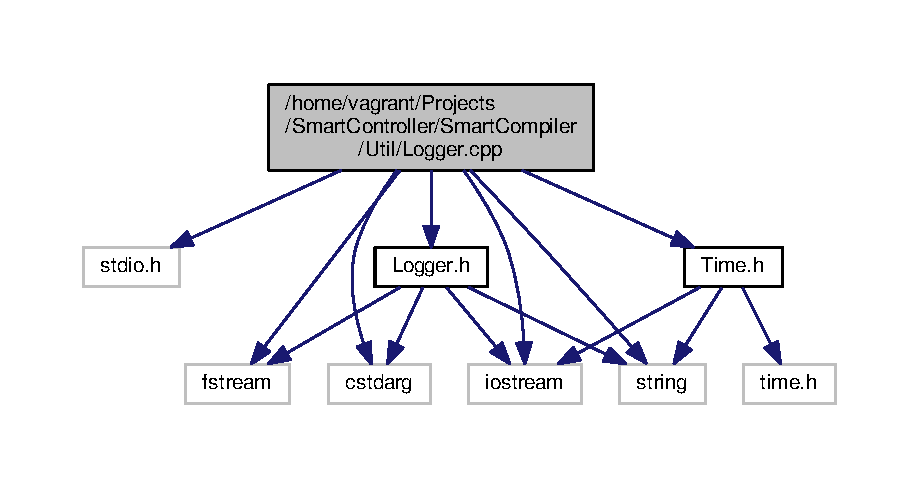
\includegraphics[width=350pt]{_logger_8cpp__incl}
\end{center}
\end{figure}
\subsection*{Namespaces}
\begin{DoxyCompactItemize}
\item 
 \hyperlink{namespace_util}{Util}
\end{DoxyCompactItemize}

\hypertarget{_logger_8h}{}\section{/home/vagrant/\+Projects/\+Smart\+Controller/\+Smart\+Compiler/\+Util/\+Logger.h File Reference}
\label{_logger_8h}\index{/home/vagrant/\+Projects/\+Smart\+Controller/\+Smart\+Compiler/\+Util/\+Logger.\+h@{/home/vagrant/\+Projects/\+Smart\+Controller/\+Smart\+Compiler/\+Util/\+Logger.\+h}}
{\ttfamily \#include $<$iostream$>$}\\*
{\ttfamily \#include $<$fstream$>$}\\*
{\ttfamily \#include $<$cstdarg$>$}\\*
{\ttfamily \#include $<$string$>$}\\*
Include dependency graph for Logger.\+h\+:\nopagebreak
\begin{figure}[H]
\begin{center}
\leavevmode
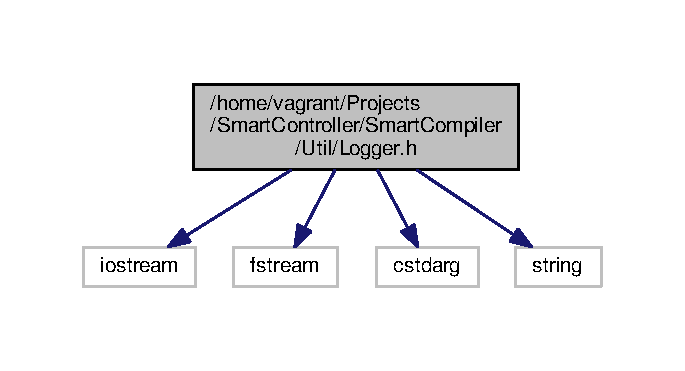
\includegraphics[width=329pt]{_logger_8h__incl}
\end{center}
\end{figure}
This graph shows which files directly or indirectly include this file\+:\nopagebreak
\begin{figure}[H]
\begin{center}
\leavevmode
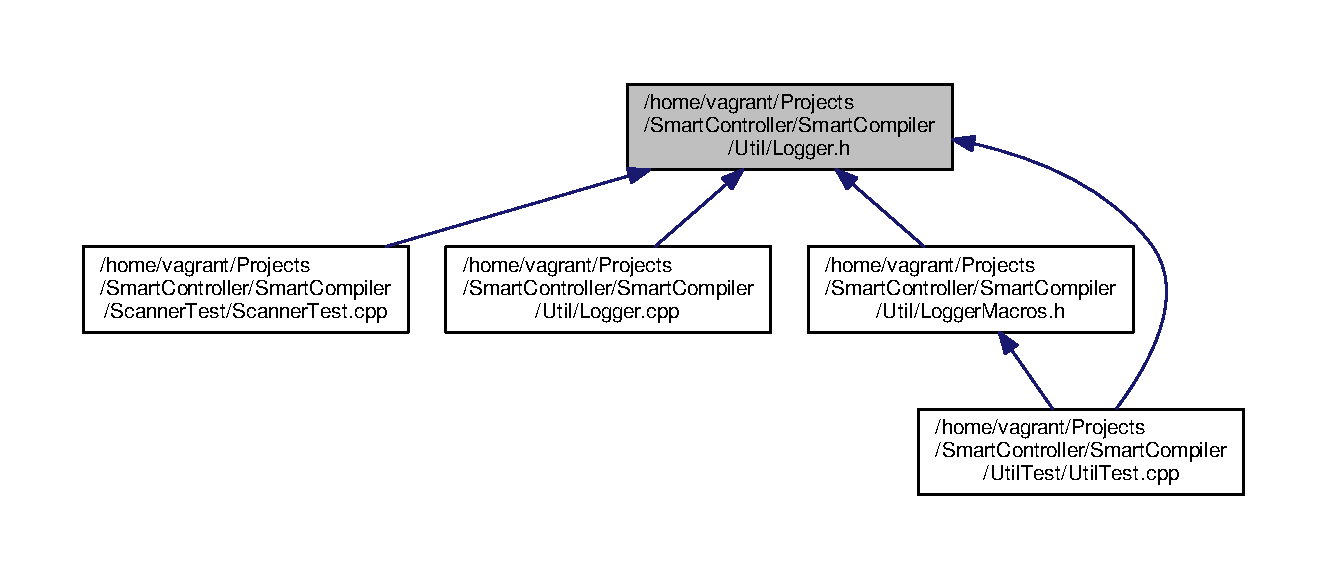
\includegraphics[width=350pt]{_logger_8h__dep__incl}
\end{center}
\end{figure}
\subsection*{Classes}
\begin{DoxyCompactItemize}
\item 
class \hyperlink{class_util_1_1_logger}{Util\+::\+Logger}
\end{DoxyCompactItemize}
\subsection*{Namespaces}
\begin{DoxyCompactItemize}
\item 
 \hyperlink{namespace_util}{Util}
\end{DoxyCompactItemize}
\subsection*{Enumerations}
\begin{DoxyCompactItemize}
\item 
enum \hyperlink{namespace_util_ae07fcfc3e173899e58af09fccd9b8b46}{Util\+::\+Msg\+Severity} \{ \hyperlink{namespace_util_ae07fcfc3e173899e58af09fccd9b8b46a3abdb59830ed7913a561b80e6451ee17}{Util\+::\+E\+R\+R\+OR}, 
\hyperlink{namespace_util_ae07fcfc3e173899e58af09fccd9b8b46af5fc0c160093801c1330b16e9bc63de6}{Util\+::\+W\+A\+R\+N\+I\+NG}, 
\hyperlink{namespace_util_ae07fcfc3e173899e58af09fccd9b8b46addebd6a35663682510acedcc15493ecd}{Util\+::\+I\+N\+FO}
 \}
\end{DoxyCompactItemize}
\subsection*{Variables}
\begin{DoxyCompactItemize}
\item 
const char $\ast$const \hyperlink{namespace_util_a7a3d115a18e867870f3f12beceb10a74}{Util\+::\+Msg\+Severity\+Text} \mbox{[}$\,$\mbox{]} = \{\char`\"{}E\+R\+R\+OR\char`\"{}, \char`\"{}W\+A\+R\+N\+I\+NG\char`\"{}, \char`\"{}I\+N\+FO\char`\"{}\}
\end{DoxyCompactItemize}

\hypertarget{_logger_macros_8h}{}\section{/home/vagrant/\+Projects/\+Smart\+Controller/\+Smart\+Compiler/\+Util/\+Logger\+Macros.h File Reference}
\label{_logger_macros_8h}\index{/home/vagrant/\+Projects/\+Smart\+Controller/\+Smart\+Compiler/\+Util/\+Logger\+Macros.\+h@{/home/vagrant/\+Projects/\+Smart\+Controller/\+Smart\+Compiler/\+Util/\+Logger\+Macros.\+h}}
{\ttfamily \#include \char`\"{}Logger.\+h\char`\"{}}\\*
Include dependency graph for Logger\+Macros.\+h\+:\nopagebreak
\begin{figure}[H]
\begin{center}
\leavevmode
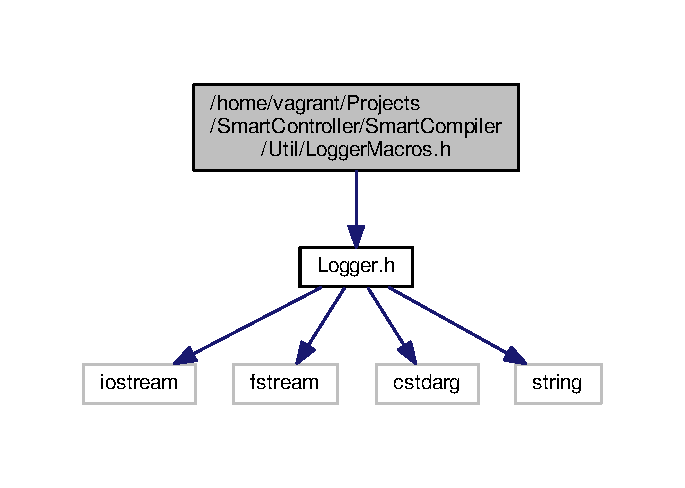
\includegraphics[width=329pt]{_logger_macros_8h__incl}
\end{center}
\end{figure}
This graph shows which files directly or indirectly include this file\+:\nopagebreak
\begin{figure}[H]
\begin{center}
\leavevmode
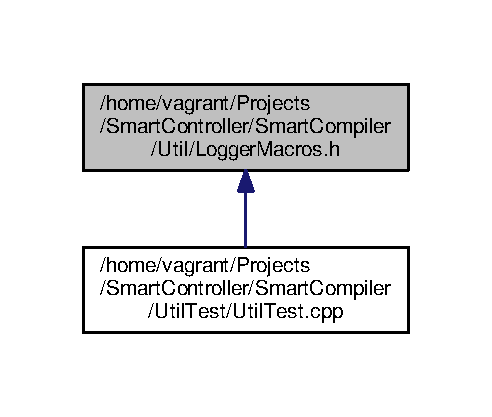
\includegraphics[width=236pt]{_logger_macros_8h__dep__incl}
\end{center}
\end{figure}
\subsection*{Macros}
\begin{DoxyCompactItemize}
\item 
\#define \hyperlink{_logger_macros_8h_a4346630e614fbede6ac716692794269f}{L\+O\+G\+E\+RR}(format, ...)
\item 
\#define \hyperlink{_logger_macros_8h_a30c1ed03d181f2cc0cc994ed08006cea}{L\+O\+G\+W\+A\+RN}(format, ...)
\item 
\#define \hyperlink{_logger_macros_8h_aaf0fa48a1b5c8dd3a598d795a1f42691}{L\+O\+G\+I\+N\+FO}(format, ...)
\end{DoxyCompactItemize}


\subsection{Macro Definition Documentation}
\index{Logger\+Macros.\+h@{Logger\+Macros.\+h}!L\+O\+G\+E\+RR@{L\+O\+G\+E\+RR}}
\index{L\+O\+G\+E\+RR@{L\+O\+G\+E\+RR}!Logger\+Macros.\+h@{Logger\+Macros.\+h}}
\subsubsection[{\texorpdfstring{L\+O\+G\+E\+RR}{LOGERR}}]{\setlength{\rightskip}{0pt plus 5cm}\#define L\+O\+G\+E\+RR(
\begin{DoxyParamCaption}
\item[{}]{format, }
\item[{}]{...}
\end{DoxyParamCaption}
)}\hypertarget{_logger_macros_8h_a4346630e614fbede6ac716692794269f}{}\label{_logger_macros_8h_a4346630e614fbede6ac716692794269f}
\index{Logger\+Macros.\+h@{Logger\+Macros.\+h}!L\+O\+G\+I\+N\+FO@{L\+O\+G\+I\+N\+FO}}
\index{L\+O\+G\+I\+N\+FO@{L\+O\+G\+I\+N\+FO}!Logger\+Macros.\+h@{Logger\+Macros.\+h}}
\subsubsection[{\texorpdfstring{L\+O\+G\+I\+N\+FO}{LOGINFO}}]{\setlength{\rightskip}{0pt plus 5cm}\#define L\+O\+G\+I\+N\+FO(
\begin{DoxyParamCaption}
\item[{}]{format, }
\item[{}]{...}
\end{DoxyParamCaption}
)}\hypertarget{_logger_macros_8h_aaf0fa48a1b5c8dd3a598d795a1f42691}{}\label{_logger_macros_8h_aaf0fa48a1b5c8dd3a598d795a1f42691}
\index{Logger\+Macros.\+h@{Logger\+Macros.\+h}!L\+O\+G\+W\+A\+RN@{L\+O\+G\+W\+A\+RN}}
\index{L\+O\+G\+W\+A\+RN@{L\+O\+G\+W\+A\+RN}!Logger\+Macros.\+h@{Logger\+Macros.\+h}}
\subsubsection[{\texorpdfstring{L\+O\+G\+W\+A\+RN}{LOGWARN}}]{\setlength{\rightskip}{0pt plus 5cm}\#define L\+O\+G\+W\+A\+RN(
\begin{DoxyParamCaption}
\item[{}]{format, }
\item[{}]{...}
\end{DoxyParamCaption}
)}\hypertarget{_logger_macros_8h_a30c1ed03d181f2cc0cc994ed08006cea}{}\label{_logger_macros_8h_a30c1ed03d181f2cc0cc994ed08006cea}

\hypertarget{_time_8h}{}\section{/home/vagrant/\+Projects/\+Smart\+Controller/\+Smart\+Compiler/\+Util/\+Time.h File Reference}
\label{_time_8h}\index{/home/vagrant/\+Projects/\+Smart\+Controller/\+Smart\+Compiler/\+Util/\+Time.\+h@{/home/vagrant/\+Projects/\+Smart\+Controller/\+Smart\+Compiler/\+Util/\+Time.\+h}}
{\ttfamily \#include $<$iostream$>$}\\*
{\ttfamily \#include $<$string$>$}\\*
{\ttfamily \#include $<$time.\+h$>$}\\*
Include dependency graph for Time.\+h\+:\nopagebreak
\begin{figure}[H]
\begin{center}
\leavevmode
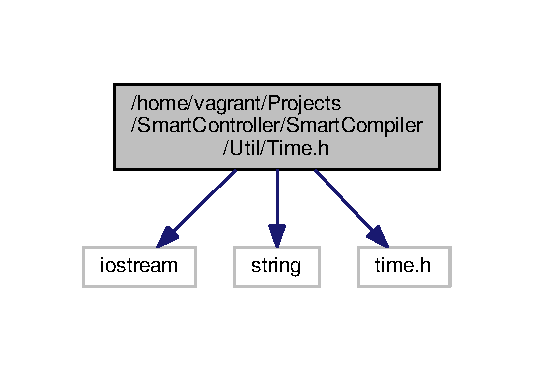
\includegraphics[width=256pt]{_time_8h__incl}
\end{center}
\end{figure}
This graph shows which files directly or indirectly include this file\+:\nopagebreak
\begin{figure}[H]
\begin{center}
\leavevmode
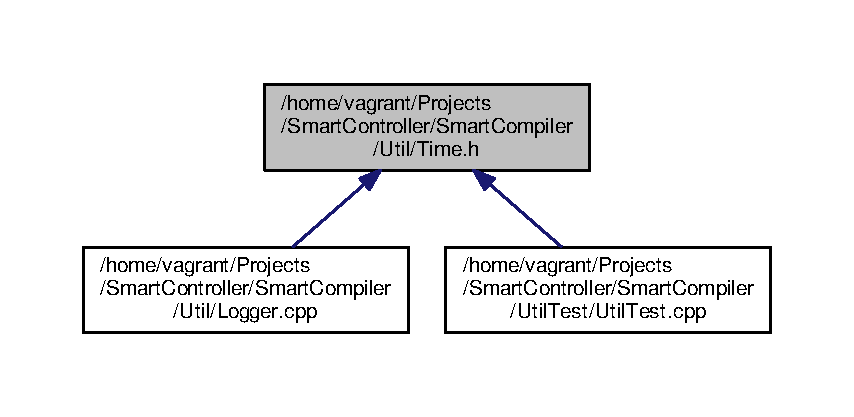
\includegraphics[width=350pt]{_time_8h__dep__incl}
\end{center}
\end{figure}
\subsection*{Namespaces}
\begin{DoxyCompactItemize}
\item 
 \hyperlink{namespace_util}{Util}
\end{DoxyCompactItemize}
\subsection*{Functions}
\begin{DoxyCompactItemize}
\item 
const string \hyperlink{namespace_util_a9fa6d22a6dbbcfc2f7def6f659036af3}{Util\+::get\+Current\+Date\+Time} ()
\begin{DoxyCompactList}\small\item\em Get current date/time,. \end{DoxyCompactList}\end{DoxyCompactItemize}
\subsection*{Variables}
\begin{DoxyCompactItemize}
\item 
constexpr short \hyperlink{namespace_util_a8dfc55b47c7119cc05aecc5eeb480e95}{Util\+::\+M\+A\+X\+\_\+\+T\+I\+M\+E\+\_\+\+B\+U\+F\+F\+ER} = 80
\end{DoxyCompactItemize}

\hypertarget{_debug_2_util_test_8d}{}\section{/home/vagrant/\+Projects/\+Smart\+Controller/\+Smart\+Compiler/\+Util\+Test/\+Debug/\+Util\+Test.d File Reference}
\label{_debug_2_util_test_8d}\index{/home/vagrant/\+Projects/\+Smart\+Controller/\+Smart\+Compiler/\+Util\+Test/\+Debug/\+Util\+Test.\+d@{/home/vagrant/\+Projects/\+Smart\+Controller/\+Smart\+Compiler/\+Util\+Test/\+Debug/\+Util\+Test.\+d}}

\hypertarget{_release_2_util_test_8d}{}\section{/home/vagrant/\+Projects/\+Smart\+Controller/\+Smart\+Compiler/\+Util\+Test/\+Release/\+Util\+Test.d File Reference}
\label{_release_2_util_test_8d}\index{/home/vagrant/\+Projects/\+Smart\+Controller/\+Smart\+Compiler/\+Util\+Test/\+Release/\+Util\+Test.\+d@{/home/vagrant/\+Projects/\+Smart\+Controller/\+Smart\+Compiler/\+Util\+Test/\+Release/\+Util\+Test.\+d}}

\hypertarget{_debug_2_util_test_main_8d}{}\section{/home/vagrant/\+Projects/\+Smart\+Controller/\+Smart\+Compiler/\+Util\+Test/\+Debug/\+Util\+Test\+Main.d File Reference}
\label{_debug_2_util_test_main_8d}\index{/home/vagrant/\+Projects/\+Smart\+Controller/\+Smart\+Compiler/\+Util\+Test/\+Debug/\+Util\+Test\+Main.\+d@{/home/vagrant/\+Projects/\+Smart\+Controller/\+Smart\+Compiler/\+Util\+Test/\+Debug/\+Util\+Test\+Main.\+d}}

\hypertarget{_release_2_util_test_main_8d}{}\section{/home/vagrant/\+Projects/\+Smart\+Controller/\+Smart\+Compiler/\+Util\+Test/\+Release/\+Util\+Test\+Main.d File Reference}
\label{_release_2_util_test_main_8d}\index{/home/vagrant/\+Projects/\+Smart\+Controller/\+Smart\+Compiler/\+Util\+Test/\+Release/\+Util\+Test\+Main.\+d@{/home/vagrant/\+Projects/\+Smart\+Controller/\+Smart\+Compiler/\+Util\+Test/\+Release/\+Util\+Test\+Main.\+d}}

\hypertarget{_util_test_8cpp}{}\section{/home/vagrant/\+Projects/\+Smart\+Controller/\+Smart\+Compiler/\+Util\+Test/\+Util\+Test.cpp File Reference}
\label{_util_test_8cpp}\index{/home/vagrant/\+Projects/\+Smart\+Controller/\+Smart\+Compiler/\+Util\+Test/\+Util\+Test.\+cpp@{/home/vagrant/\+Projects/\+Smart\+Controller/\+Smart\+Compiler/\+Util\+Test/\+Util\+Test.\+cpp}}
{\ttfamily \#include \char`\"{}Time.\+h\char`\"{}}\\*
{\ttfamily \#include \char`\"{}Logger.\+h\char`\"{}}\\*
{\ttfamily \#include \char`\"{}Logger\+Macros.\+h\char`\"{}}\\*
{\ttfamily \#include \char`\"{}Util\+Test.\+h\char`\"{}}\\*
Include dependency graph for Util\+Test.\+cpp\+:\nopagebreak
\begin{figure}[H]
\begin{center}
\leavevmode
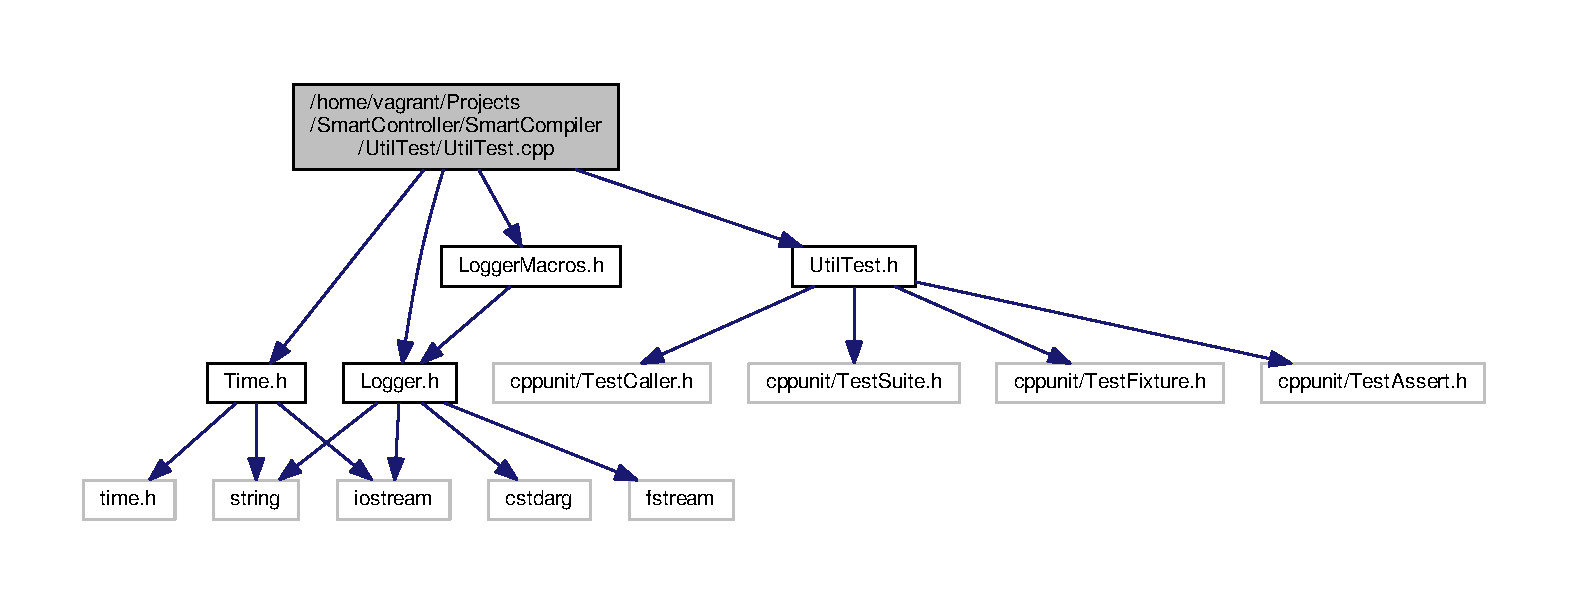
\includegraphics[width=350pt]{_util_test_8cpp__incl}
\end{center}
\end{figure}
\subsection*{Namespaces}
\begin{DoxyCompactItemize}
\item 
 \hyperlink{namespace_util}{Util}
\end{DoxyCompactItemize}

\hypertarget{_util_test_8h}{}\section{/home/vagrant/\+Projects/\+Smart\+Controller/\+Smart\+Compiler/\+Util\+Test/\+Util\+Test.h File Reference}
\label{_util_test_8h}\index{/home/vagrant/\+Projects/\+Smart\+Controller/\+Smart\+Compiler/\+Util\+Test/\+Util\+Test.\+h@{/home/vagrant/\+Projects/\+Smart\+Controller/\+Smart\+Compiler/\+Util\+Test/\+Util\+Test.\+h}}
{\ttfamily \#include $<$cppunit/\+Test\+Fixture.\+h$>$}\\*
{\ttfamily \#include $<$cppunit/\+Test\+Assert.\+h$>$}\\*
{\ttfamily \#include $<$cppunit/\+Test\+Caller.\+h$>$}\\*
{\ttfamily \#include $<$cppunit/\+Test\+Suite.\+h$>$}\\*
Include dependency graph for Util\+Test.\+h\+:\nopagebreak
\begin{figure}[H]
\begin{center}
\leavevmode
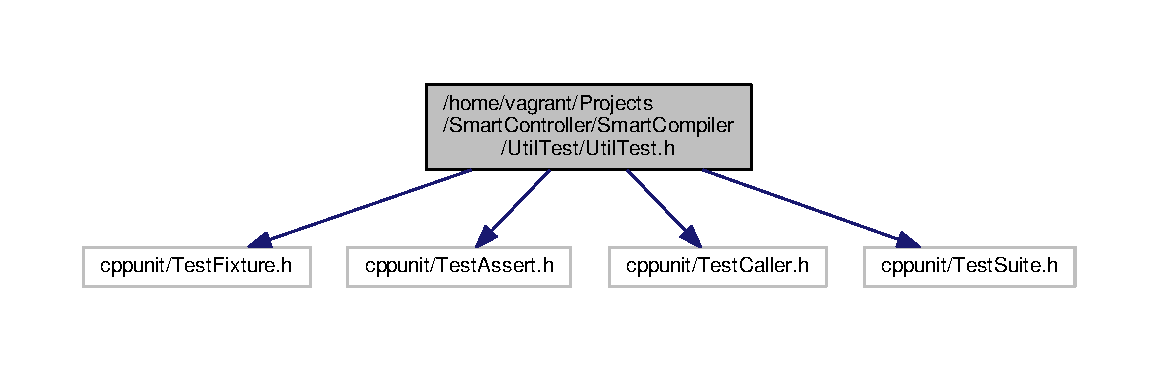
\includegraphics[width=350pt]{_util_test_8h__incl}
\end{center}
\end{figure}
This graph shows which files directly or indirectly include this file\+:\nopagebreak
\begin{figure}[H]
\begin{center}
\leavevmode
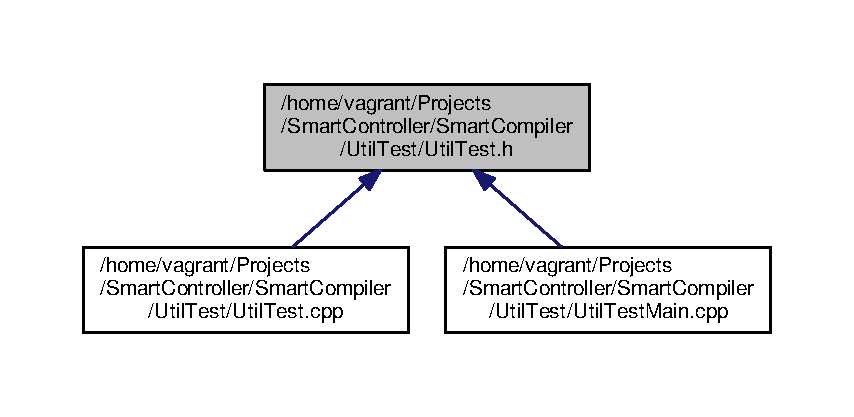
\includegraphics[width=350pt]{_util_test_8h__dep__incl}
\end{center}
\end{figure}
\subsection*{Classes}
\begin{DoxyCompactItemize}
\item 
class \hyperlink{class_util_1_1_util_test}{Util\+::\+Util\+Test}
\end{DoxyCompactItemize}
\subsection*{Namespaces}
\begin{DoxyCompactItemize}
\item 
 \hyperlink{namespace_util}{Util}
\end{DoxyCompactItemize}

\hypertarget{_util_test_main_8cpp}{}\section{/home/vagrant/\+Projects/\+Smart\+Controller/\+Smart\+Compiler/\+Util\+Test/\+Util\+Test\+Main.cpp File Reference}
\label{_util_test_main_8cpp}\index{/home/vagrant/\+Projects/\+Smart\+Controller/\+Smart\+Compiler/\+Util\+Test/\+Util\+Test\+Main.\+cpp@{/home/vagrant/\+Projects/\+Smart\+Controller/\+Smart\+Compiler/\+Util\+Test/\+Util\+Test\+Main.\+cpp}}
{\ttfamily \#include $<$iostream$>$}\\*
{\ttfamily \#include $<$cppunit/\+Test\+Suite.\+h$>$}\\*
{\ttfamily \#include $<$cppunit/ui/text/\+Test\+Runner.\+h$>$}\\*
{\ttfamily \#include \char`\"{}Util\+Test.\+h\char`\"{}}\\*
Include dependency graph for Util\+Test\+Main.\+cpp\+:\nopagebreak
\begin{figure}[H]
\begin{center}
\leavevmode
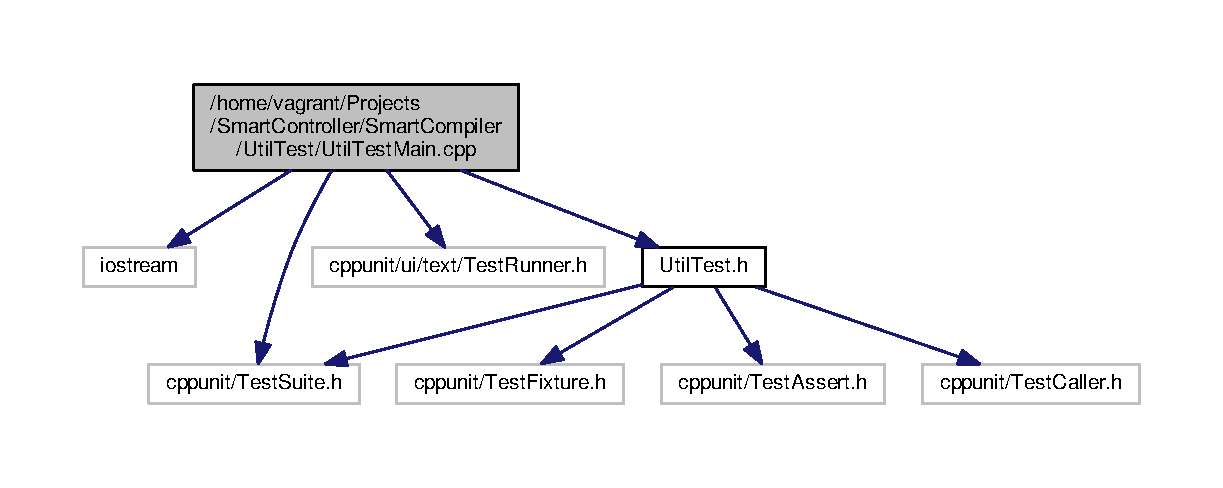
\includegraphics[width=350pt]{_util_test_main_8cpp__incl}
\end{center}
\end{figure}
\subsection*{Functions}
\begin{DoxyCompactItemize}
\item 
int \hyperlink{_util_test_main_8cpp_ae66f6b31b5ad750f1fe042a706a4e3d4}{main} ()
\end{DoxyCompactItemize}


\subsection{Function Documentation}
\index{Util\+Test\+Main.\+cpp@{Util\+Test\+Main.\+cpp}!main@{main}}
\index{main@{main}!Util\+Test\+Main.\+cpp@{Util\+Test\+Main.\+cpp}}
\subsubsection[{\texorpdfstring{main()}{main()}}]{\setlength{\rightskip}{0pt plus 5cm}int main (
\begin{DoxyParamCaption}
{}
\end{DoxyParamCaption}
)}\hypertarget{_util_test_main_8cpp_ae66f6b31b5ad750f1fe042a706a4e3d4}{}\label{_util_test_main_8cpp_ae66f6b31b5ad750f1fe042a706a4e3d4}

%--- End generated contents ---

% Index
\backmatter
\newpage
\phantomsection
\clearemptydoublepage
\addcontentsline{toc}{chapter}{Index}
\printindex

\end{document}
